% !TEX program = xelatex
\documentclass[12pt, a4paper, oneside]{book}
% !TEX root = ../do-an.tex
% =====================================================================
%  styles/settings.tex
%  Các thiết lập chung, nạp từ file chính do-an.tex.
%  SINH VIÊN KHÔNG SỬA FILE NÀY.
%
%  Lưu ý: lệnh khai báo lớp tài liệu nằm ở file do-an.tex chứ không nằm
%  ở đây. Lý do: Overleaf dò file chính bằng cách tìm chuỗi khai báo lớp
%  tài liệu trong các file. Nếu chuỗi đó xuất hiện ở file này, Overleaf
%  sẽ biên dịch nhầm file này và báo lỗi "no legal end found", vì file
%  này chỉ chứa thiết lập chứ không chứa phần thân tài liệu.
% =====================================================================

% Toàn bộ nhận diện DAU: phông, màu, bìa, hộp trình bày, header
\usepackage{styles/dau}
\dauLayout

% Giãn dòng và khoảng cách đoạn theo quy cách đồ án
\linespread{1.25}
\usepackage[skip=8pt plus 1pt, indent=15pt]{parskip}

% Ghi chú: mẫu gốc dùng gói atbegshi để vứt trang đầu, vì trang bìa của
% mẫu gốc dựng bằng minipage nên sinh ra một trang trắng. Trang bìa ở
% đây dựng bằng môi trường titlepage nên không có trang trắng, và nếu
% giữ thủ thuật đó thì chính trang bìa sẽ bị vứt mất.

\usepackage{longtable}

% Thông tin bìa: thay các giá trị trong ngoặc vuông trước khi nộp.
\crname{BÁO CÁO ĐỒ ÁN TRÍ TUỆ NHÂN TẠO}
\cmonhoc{Học phần AIP202 \textperiodcentered{} 2 tín chỉ}
\ctname{XÂY DỰNG HỆ THỐNG GỢI Ý VÀ\\TÌM KIẾM CÔNG THỨC NẤU ĂN}
\cstuname{NGUYỄN HỮU PHÚC}
\cmssv{2351220005}
\clopsv{23CT1}
\csCouncil{Công nghệ thông tin}
\csSupervise{TS. Đỗ Phúc Hảo}
\cttime{2026--2027}
\csdeptname{KHOA CÔNG NGHỆ THÔNG TIN}
\csplace{Đà Nẵng}

\begin{document}
\coverpage

\frontmatter
\dauPageStyle
\begin{declaration}

Tôi cam đoan báo cáo này phản ánh đúng sản phẩm và các kết quả kiểm thử của
đồ án \emph{Xây dựng hệ thống gợi ý và tìm kiếm công thức nấu ăn}. Những số
liệu về dữ liệu, mô hình, công thức và phần mềm đều được đối chiếu với mã
nguồn hoặc tệp kết quả kèm theo. Các tài liệu, mô hình tiền huấn luyện, bộ dữ
liệu, công thức và hình ảnh của bên thứ ba đều được ghi nguồn trong báo cáo.

Trong quá trình thực hiện, công cụ trí tuệ nhân tạo được sử dụng để hỗ trợ
tra cứu, rà soát mã nguồn, gợi ý cách trình bày và kiểm tra tài liệu. Tôi chịu
trách nhiệm kiểm chứng nội dung, hiểu giải pháp và giải thích được toàn bộ hệ
thống. Công cụ hỗ trợ không thay thế trách nhiệm học thuật của người thực hiện.

Tôi chịu trách nhiệm về tính trung thực của báo cáo và sản phẩm đồ án.

\vspace{2cm}
\begin{flushright}
Đà Nẵng, ngày \ldots{} tháng \ldots{} năm \ldots{}\\[1.5cm]
\textbf{Sinh viên thực hiện}\\[1.5cm]
\textbf{\dauSinhVien}
\end{flushright}

\end{declaration}

\begin{acknowledgments}

Tôi xin chân thành cảm ơn giảng viên hướng dẫn đã góp ý về phạm vi, phương
pháp thực hiện và cách đánh giá đồ án. Tôi cũng cảm ơn các giảng viên Khoa
Công nghệ Thông tin đã cung cấp kiến thức nền tảng về lập trình, cơ sở dữ
liệu, phát triển ứng dụng và trí tuệ nhân tạo.

Đồ án sử dụng các tài nguyên mở và công cụ do cộng đồng phát triển, gồm
Flutter, FastAPI, PyTorch, Transformers, SQLite, bộ dữ liệu 30VNFoods và mô
hình nhận diện món Việt được công bố trên Hugging Face. Tôi trân trọng ghi
nhận đóng góp của các tác giả và cộng đồng duy trì những tài nguyên này.

Do giới hạn thời gian và kinh nghiệm, báo cáo khó tránh khỏi thiếu sót. Tôi
mong nhận được góp ý để tiếp tục hoàn thiện hệ thống.

\vspace{2cm}
\begin{flushright}
\textbf{\dauSinhVien}
\end{flushright}

\end{acknowledgments}

\begin{abstract}

Ẩm thực Việt Nam đa dạng theo vùng miền, trong khi người dùng đôi khi chỉ có
ảnh món ăn mà không biết tên để tìm công thức phù hợp. Đồ án xây dựng hệ
thống Vị Việt nhằm kết hợp khám phá công thức có nguồn với nhận diện món ăn
từ ảnh trên thiết bị di động. Ứng dụng Flutter giao tiếp với backend FastAPI
qua HTTP; dữ liệu nghiệp vụ được lưu bằng SQLite và SQLAlchemy. Ảnh JPEG hoặc
PNG được xử lý bởi mô hình Vision Transformer ViT-L/16 tiền huấn luyện, sau
đó nhãn dự đoán được chuẩn hóa và ánh xạ tới bản ghi món ăn trong cơ sở dữ
liệu. Hệ thống hiện quản lý 38 món đã xuất bản, 38 ảnh có metadata giấy phép,
348 nguyên liệu, 205 bước nấu và 85 nguồn tham khảo. Tám công thức được dịch
và chuẩn hóa từ nguồn mở; ba mươi công thức còn lại do Vị Việt biên soạn và
đối chiếu tối thiểu hai nguồn. Bộ dữ liệu 30VNFoods gồm 25.136 ảnh thuộc 30
lớp được audit và tạo manifest sạch còn 25.032 ảnh; tập kiểm thử sạch gồm
5.014 ảnh được dùng để đánh giá độc lập 30 lớp giao nhau với model. Ngoài
nhận diện, ứng dụng hỗ trợ tìm kiếm, lọc, yêu thích, lịch sử, phản hồi kết
quả và hiển thị nguồn--bản quyền. Hệ thống chứng minh khả năng kết hợp mô
hình thị giác tiền huấn luyện với một kho công thức có thể truy nguyên trong
một ứng dụng mobile hoàn chỉnh, đồng thời chỉ rõ giới hạn khi tập đánh giá
chưa bao phủ đủ 38 nhãn của model.

\vspace{0.8em}
\noindent\textbf{Từ khoá:} nhận diện món ăn, Vision Transformer, Flutter,
FastAPI, công thức món Việt, 30VNFoods.

\end{abstract}

\chapter*{Danh mục từ viết tắt}
\addcontentsline{toc}{chapter}{Danh mục từ viết tắt}

\begin{table}[htbp]
\centering
\begin{tabular*}{\textwidth}{@{\extracolsep{\fill}}>{\bfseries\color{daumaroon}}l l}
\toprule
API & Application Programming Interface -- giao diện lập trình ứng dụng \\
AI & Artificial Intelligence -- trí tuệ nhân tạo \\
ERD & Entity--Relationship Diagram -- sơ đồ thực thể--liên kết \\
HTTP & Hypertext Transfer Protocol \\
JWT & JSON Web Token \\
ORM & Object--Relational Mapping \\
RGB & Red, Green, Blue \\
UI/UX & User Interface/User Experience \\
ViT & Vision Transformer \\
\bottomrule
\end{tabular*}
\end{table}

\tableofcontents
\listoffigures
\listoftables
\listofalgorithms

\mainmatter
\dauPageStyle
\chapter{Mở đầu}
\label{ch:modau}

\begin{muctieu}
Chương này trình bày bối cảnh, vấn đề cần giải quyết, mục tiêu đo lường được,
phạm vi và bố cục của đồ án Vị Việt.
\end{muctieu}

\section{Lý do chọn đề tài}

Ẩm thực Việt Nam có số lượng món lớn, tên gọi và biến thể khác nhau theo vùng
miền. Khi bắt gặp một món ăn qua ảnh, người dùng có thể không biết tên chính
xác để tìm kiếm. Ngược lại, kết quả tìm kiếm trên Internet thường phân tán,
khó phân biệt nội dung có nguồn với nội dung được sao chép hoặc tạo tự động.
Hai khó khăn này tạo ra nhu cầu về một hệ thống vừa nhận diện món qua ảnh,
vừa dẫn người dùng đến công thức có thể truy nguyên.

Nhận diện món ăn là một bài toán phân loại ảnh nhiều lớp. Food-101 cho thấy
đây là bài toán khó do sự khác biệt lớn về cách trình bày, ánh sáng và nền
ảnh, đồng thời nhiều món có hình thức gần giống nhau
\cite{bossard2014food101}. Với món Việt, 30VNFoods cung cấp 25.136 ảnh thuộc
30 lớp và là nguồn phù hợp để đánh giá model trong phạm vi đề tài
\cite{do2021_30vnfoods}. Đồ án chọn cách khai thác mô hình ViT tiền huấn luyện
thay vì huấn luyện mạng mới từ đầu, nhờ đó tập trung nguồn lực vào tích hợp
hệ thống, chất lượng dữ liệu công thức và trải nghiệm mobile.

Sản phẩm được đặt tên \term{Vị Việt}, hướng đến trải nghiệm tối giản: người
dùng có thể tìm món bằng chữ hoặc chụp/chọn ảnh, xem kết quả Top~1 kèm độ tin
cậy, rồi mở đúng công thức tương ứng. Công thức và ảnh chỉ được xuất bản khi
có metadata nguồn và giấy phép hợp lệ.

\section{Mục tiêu của đồ án}

Đồ án hướng tới các mục tiêu cụ thể sau:
\begin{itemize}
  \item Xây dựng ứng dụng Flutter chạy trên Android, hỗ trợ chế độ khách,
        đăng ký, đăng nhập và quản lý phiên.
  \item Tích hợp model ViT-L/16 gồm 38 nhãn món Việt; hỗ trợ ảnh JPEG/PNG,
        trả tên món, độ tin cậy và dữ liệu món được ánh xạ từ database.
  \item Cung cấp danh mục 38 món có ảnh, nguyên liệu, bước nấu, thời gian,
        khẩu phần, nguồn công thức và metadata giấy phép.
  \item Hỗ trợ tìm kiếm, lọc, yêu thích, lịch sử nhận diện, phản hồi nhãn
        đúng và chỉnh sửa tên tài khoản.
  \item Xây dựng backend FastAPI có kiểm tra đầu vào, xác thực JWT, migration,
        audit dữ liệu và tài liệu OpenAPI.
  \item Đánh giá model trên toàn bộ 5.014 ảnh thuộc tập Test sạch của 30 lớp
        giao nhau giữa 30VNFoods và model; báo cáo trung thực giới hạn tám
        nhãn chưa được bộ dữ liệu này bao phủ.
\end{itemize}

\section{Đối tượng sử dụng}

Đối tượng chính là người quan tâm tới món ăn Việt và muốn khám phá công thức
bằng tên món hoặc hình ảnh. Khách có thể xem danh mục, tìm kiếm và nhận diện.
Người dùng đăng nhập có thêm khả năng lưu yêu thích, xem/xóa lịch sử và gửi
phản hồi khi kết quả chưa đúng. Đối tượng kỹ thuật gồm người quản lý dữ liệu
công thức và lập trình viên cần audit, import hoặc triển khai lại hệ thống.

\section{Phạm vi và giới hạn}

Phạm vi nhận diện được giới hạn ở 38 nhãn trong cấu hình model. Giao diện chỉ
hiển thị Top~1 để tối giản; backend vẫn lưu Top~3 cho lịch sử và đánh giá. Ảnh
người dùng chỉ được giữ trong bộ nhớ trong lúc suy luận, không được ghi vào ổ
đĩa hoặc database. Đồ án chưa huấn luyện lại model production, chưa triển khai
backend công khai và chưa tối ưu cho nhiều API instance. SQLite phù hợp với
demo đơn máy nhưng không thay thế hệ quản trị cơ sở dữ liệu cho production.

Dataset 30VNFoods là dữ liệu ảnh phục vụ audit và đánh giá, không phải database
công thức. Tám nhãn model không xuất hiện trong dataset nên các độ đo trên tập
Test chỉ phản ánh 30 lớp giao nhau. Công thức được biên soạn hoặc dịch từ nguồn
có thể truy nguyên, nhưng không được tuyên bố là nội dung đã qua chuyên gia ẩm
thực kiểm duyệt.

\section{Bố cục báo cáo}

Phần còn lại của báo cáo được tổ chức như sau. Chương~\ref{ch:coso} trình
bày cơ sở lý thuyết và công nghệ. Chương~\ref{ch:thietke} phân tích yêu cầu
và thiết kế hệ thống. Chương~\ref{ch:caidat} mô tả quá trình cài đặt, dữ liệu,
giao diện và kiểm thử. Chương~\ref{ch:ketqua} trình bày kết quả đánh giá,
bàn luận và hạn chế. Chương~\ref{ch:ketluan} tổng kết và đề xuất hướng phát
triển.

\chapter{Cơ sở lý thuyết và công nghệ}
\label{ch:coso}

\begin{muctieu}
Chương này tóm lược những khái niệm trực tiếp được sử dụng trong hệ thống:
phân loại ảnh, Transformer, Vision Transformer, các độ đo đánh giá và nền
tảng phần mềm triển khai.
\end{muctieu}

\section{Bài toán phân loại ảnh nhiều lớp}

Với ảnh đầu vào $x$ và tập nhãn hữu hạn $\mathcal{Y}=\{1,\ldots,K\}$, bộ
phân loại học hàm $f:x\mapsto y$ để chọn một nhãn $y\in\mathcal{Y}$. Trong
đồ án, $K=38$ và mỗi nhãn biểu diễn một món ăn. Model sinh vector điểm thô
$\mathbf{z}\in\mathbb{R}^{K}$. Xác suất lớp $k$ được tính bằng Softmax:
\begin{equation}
p(y=k\mid x)=\frac{\exp(z_k)}{\sum_{j=1}^{K}\exp(z_j)}.
\label{eq:softmax}
\end{equation}
Nhãn có xác suất lớn nhất là Top~1; ba nhãn lớn nhất tạo thành Top~3. Xác
suất cao không đồng nghĩa chắc chắn tuyệt đối, vì model vẫn có thể tự tin ở
ảnh ngoài phân phối hoặc các món có hình thức gần nhau.

\section{Transformer và cơ chế tự chú ý}

Transformer thay thế xử lý tuần tự bằng cơ chế self-attention, cho phép mỗi
token tổng hợp thông tin từ các token khác \cite{vaswani2017attention}. Với
ma trận truy vấn $Q$, khóa $K$ và giá trị $V$, scaled dot-product attention
được tính theo:
\begin{equation}
\operatorname{Attention}(Q,K,V)=
\operatorname{softmax}\left(\frac{QK^{\mathsf T}}{\sqrt{d_k}}\right)V,
\label{eq:attention}
\end{equation}
trong đó $d_k$ là số chiều của vector khóa. Multi-head attention thực hiện
nhiều phép attention song song để học các quan hệ khác nhau.

\section{Vision Transformer}

Vision Transformer (ViT) chia ảnh thành các patch không chồng lấn, biến mỗi
patch thành một token, thêm positional embedding và token phân lớp
\cite{dosovitskiy2021vit}. Ảnh 384$\times$384 với patch 16$\times$16 tạo
ra $24\times24=576$ patch. Chuỗi 576 token ảnh cùng token phân lớp đi qua 24
Transformer encoder của cấu hình ViT-L/16. Vector ở token phân lớp được đưa
vào lớp tuyến tính để sinh logits cho 38 món.

ViT tận dụng tốt học chuyển giao khi được tiền huấn luyện trên dữ liệu lớn.
Đồ án dùng model \code{VietTung04/vit-l-16-food-classifier}, một phiên bản
ViT-L/16 đã được fine-tune cho món Việt và công bố theo giấy phép Apache-2.0
\cite{vietTungModel}. Model được tải một lần, lưu local và chạy ở chế độ
\code{eval} kết hợp \code{torch.inference\_mode}.

\section{Các độ đo đánh giá}

Với mỗi lớp, $TP$, $FP$ và $FN$ lần lượt là số dự đoán đúng, dương tính giả
và âm tính giả. Các độ đo được tính theo:
\begin{align}
\mathrm{Accuracy} &= \frac{\text{số dự đoán đúng}}{\text{tổng số mẫu}},\\
\mathrm{Precision} &= \frac{TP}{TP+FP},\\
\mathrm{Recall} &= \frac{TP}{TP+FN},\\
F_1 &= \frac{2\,\mathrm{Precision}\,\mathrm{Recall}}
{\mathrm{Precision}+\mathrm{Recall}}.
\end{align}
Macro average là trung bình không trọng số của 30 lớp đánh giá, nhờ đó mỗi
lớp có đóng góp ngang nhau dù số ảnh khác nhau. Ma trận nhầm lẫn cho biết các
cặp lớp model thường dự đoán lẫn nhau.

\section{Kiến trúc client--server và REST API}

Ứng dụng Flutter đóng vai trò client, còn FastAPI cung cấp tài nguyên qua
HTTP/JSON và nhận ảnh dưới dạng multipart. FastAPI dựa trên chuẩn OpenAPI và
tự sinh Swagger UI, thuận tiện cho kiểm thử contract \cite{fastapiDocs}.
Flutter khuyến nghị tách UI, trạng thái, repository và service để giảm phụ
thuộc và tăng khả năng kiểm thử \cite{flutterArchitecture}. Dự án hiện dùng
screen/widget ở lớp UI, \code{AppState} cho trạng thái và \code{ApiClient}
cùng \code{AiService} cho lớp dữ liệu.

\section{Lưu trữ và bảo mật}

SQLite là database nhúng, serverless, giao dịch và lưu toàn bộ dữ liệu trong
một tệp \cite{sqliteAbout}. SQLAlchemy ánh xạ lớp Python sang bảng quan hệ,
quản lý session, transaction và relationship \cite{sqlalchemyDocs}. Mật khẩu
được băm bằng Argon2, một hàm memory-hard được mô tả trong RFC~9106
\cite{rfc9106}. Access token và refresh token tuân theo cấu trúc JWT của
RFC~7519 \cite{rfc7519}; refresh token còn có phiên trong database để hỗ trợ
xoay vòng và thu hồi.

\section{Công cụ và thư viện}

\begin{table}[htbp]
\centering
\caption{Các thành phần chính của hệ thống.}
\label{tab:congcu}
\small
\begin{tabularx}{\textwidth}{>{\bfseries\color{daunavy}}l >{\color{daumaroon}}l X}
\toprule
\textbf{Thành phần} & \textbf{Phiên bản kiểm chứng} & \textbf{Vai trò} \\
\midrule
Flutter & 3.47.2 & Ứng dụng mobile đa nền tảng \\
Dart & 3.13.x & Ngôn ngữ của Flutter \\
Python & 3.13.7 & Backend, audit và suy luận AI \\
FastAPI & 0.141.1 & REST API, validation và OpenAPI \\
PyTorch & 2.14.0+cpu & Tensor và suy luận model \cite{paszke2019pytorch} \\
Transformers & 5.17.0 & Processor và ViT \cite{huggingfaceTransformers} \\
SQLAlchemy & 2.1.3 & ORM và transaction \\
SQLite & 3.x & Database cục bộ \\
Android Studio & Bản cài hiện tại & Emulator, build và chạy Flutter \\
\bottomrule
\end{tabularx}
\end{table}

Phiên bản trong Bảng~\ref{tab:congcu} mô tả môi trường đã kiểm chứng của đồ
án; giới hạn dependency chính xác vẫn được quản lý trong
\code{requirements.txt} và \code{pubspec.yaml}.

\section{Dữ liệu và các công trình liên quan}

Food-101 đặt nền móng cho đánh giá nhận diện món ăn quy mô lớn với 101.000
ảnh thuộc 101 lớp \cite{bossard2014food101}. 30VNFoods tập trung vào 30 món
Việt và công bố 25.136 ảnh \cite{do2021_30vnfoods}. Model sử dụng trong đồ
án kế thừa ViT-L/16 và được tác giả model fine-tune trên 30VNFoods kết hợp dữ
liệu tự thu thập \cite{vietTungModel}. Khác với công trình chỉ tập trung phân
loại, Vị Việt tích hợp model vào luồng ứng dụng có xác thực, lịch sử, phản
hồi và kho công thức có metadata nguồn.

Với dữ liệu công thức, tám món được dịch và chuẩn hóa từ Wikibooks theo điều
kiện CC BY-SA 4.0 \cite{wikibooksCopyright}. Ảnh giao diện được chọn theo
metadata riêng của từng tệp trên Wikimedia Commons/Openverse; việc sử dụng
ảnh tuân theo yêu cầu attribution và giấy phép của tệp \cite{commonsReuse}.

\chapter{Phân tích và thiết kế}
\label{ch:thietke}

\begin{muctieu}
Chương này phân tích yêu cầu của Vị Việt, mô tả kiến trúc, dữ liệu, luồng
nhận diện và cấu hình model được tích hợp trong sản phẩm.
\end{muctieu}

\section{Phân tích bài toán}

Hệ thống cần giải quyết hai đường vào cùng hội tụ về một kho công thức. Với
tìm kiếm văn bản, người dùng nhập tên hoặc từ khóa; backend chuẩn hóa chuỗi
và trả danh sách món phù hợp. Với nhận diện ảnh, client gửi JPEG/PNG; model
sinh nhãn, backend chuẩn hóa nhãn đó rồi tìm bản ghi \code{dishes}. Đầu ra
cuối cùng là món chuẩn, ảnh minh họa, thời gian, khẩu phần, nguyên liệu, các
bước thực hiện và metadata nguồn.

Hai nhóm tác nhân được trình bày ở Hình~\ref{fig:usecase}. Khách sử dụng các
chức năng không cá nhân hóa. Người dùng đăng nhập có thêm yêu thích, lịch sử,
phản hồi và hồ sơ. Không có trang quản trị trong phạm vi đồ án; dữ liệu công
thức được cập nhật bằng catalog JSON và importer có kiểm tra.

\begin{figure}[htbp]
\centering
\resizebox{0.94\textwidth}{!}{\begin{tikzpicture}[x=1cm,y=1cm,
  actor/.style={rectangle, rounded corners=3pt, draw=daunavy,
    line width=.9pt, fill=lightnavy, minimum width=2.7cm,
    minimum height=10mm, align=center, font=\footnotesize, soft},
  usecase/.style={ellipse, draw=daumaroon, line width=.8pt, fill=white,
    minimum width=4.0cm, minimum height=10mm, align=center,
    font=\footnotesize}]
  \node[actor] (guest) at (-4.4,1.8) {Khách};
  \node[actor] (member) at (-4.4,-2.0) {Người dùng\\đăng nhập};

  \node[usecase] (browse) at (0,2.7) {Xem/tìm kiếm công thức};
  \node[usecase] (detail) at (0,1.2) {Xem chi tiết và nguồn};
  \node[usecase] (predict) at (0,-0.3) {Nhận diện món từ ảnh};
  \node[usecase] (auth) at (0,-1.8) {Đăng ký/đăng nhập};

  \node[usecase] (favorite) at (5.2,2.7) {Quản lý yêu thích};
  \node[usecase] (history) at (5.2,1.2) {Xem/xóa lịch sử};
  \node[usecase] (feedback) at (5.2,-0.3) {Gửi phản hồi nhãn đúng};
  \node[usecase] (profile) at (5.2,-1.8) {Sửa tên/đăng xuất};

  \node[draw=gray300, rounded corners=5pt, inner sep=8mm,
        fit=(browse)(profile), label={[font=\small\bfseries,
        text=daunavy]above:Hệ thống Vị Việt}] (system) {};

  \coordinate (guestbus) at (-2.55,1.8);
  \coordinate (memberbus) at (2.6,-3.0);
  \draw[assoc] (guest.east) -- (guestbus);
  \draw[assoc] (guestbus) |- (browse.west);
  \draw[assoc] (guestbus) |- (detail.west);
  \draw[assoc] (guestbus) |- (predict.west);
  \draw[assoc] (guestbus) |- (auth.west);

  \draw[assoc, -{Triangle[open,length=2.7mm,width=2.2mm]}]
    (member.north) -- (guest.south);
  \draw[assoc] (member.east) -- ++(1.1,0) |- (memberbus);
  \draw[assoc] (memberbus) |- (favorite.south);
  \draw[assoc] (memberbus) |- (history.south);
  \draw[assoc] (memberbus) |- (feedback.south);
  \draw[assoc] (memberbus) |- (profile.south);
\end{tikzpicture}
}
\caption{Sơ đồ Use Case tổng thể của Vị Việt.}
\label{fig:usecase}
\end{figure}

\section{Yêu cầu chức năng}

\begin{table}[htbp]
\centering
\caption{Các yêu cầu chức năng chính.}
\label{tab:functional-requirements}
\small
\begin{tabularx}{\textwidth}{>{\bfseries\color{daumaroon}}l X >{\centering\arraybackslash}p{2.2cm}}
\toprule
Mã & Mô tả & Tác nhân \\
\midrule
FR01 & Đăng ký, đăng nhập, refresh token và đăng xuất. & Người dùng \\
FR02 & Xem, tìm kiếm và lọc danh mục món. & Tất cả \\
FR03 & Xem chi tiết công thức, nguồn và giấy phép. & Tất cả \\
FR04 & Chụp/chọn ảnh, gửi nhận diện và xem Top~1. & Tất cả \\
FR05 & Mở trực tiếp công thức của món đã nhận diện. & Tất cả \\
FR06 & Thêm hoặc bỏ món yêu thích. & Đăng nhập \\
FR07 & Xem, xóa lịch sử và gửi phản hồi nhãn đúng. & Đăng nhập \\
FR08 & Đọc hồ sơ và thay đổi họ tên. & Đăng nhập \\
\bottomrule
\end{tabularx}
\end{table}

\section{Yêu cầu phi chức năng}

\begin{itemize}
  \item \textbf{Đúng dữ liệu:} không xuất bản công thức khi thiếu nguồn,
        nguyên liệu, bước nấu hoặc metadata ảnh.
  \item \textbf{Bảo mật:} mật khẩu băm Argon2; JWT có hạn dùng; refresh token
        xoay vòng và có thể thu hồi; secret production phải đủ mạnh.
  \item \textbf{Quyền riêng tư:} ảnh nhận diện không được lưu; lịch sử chỉ
        lưu nhãn, confidence, Top~3 và thời điểm.
  \item \textbf{Khả dụng:} giao diện tiếng Việt, vùng chạm đủ lớn, có trạng
        thái loading, lỗi, rỗng và fallback ảnh.
  \item \textbf{Tương thích:} Android Emulator dùng \code{10.0.2.2}; URL
        thiết bị thật cấu hình bằng \code{API\_BASE\_URL}.
  \item \textbf{Bảo trì:} database có migration; importer idempotent theo
        slug; model và dataset tách khỏi Git.
\end{itemize}

\section{Luồng nhận diện món ăn}

Hình~\ref{fig:activity} mô tả toàn bộ luồng từ lúc chọn ảnh đến khi mở công
thức. Ảnh sai định dạng hoặc không giải mã được bị chặn trước khi suy luận.
Nếu nhãn model không ánh xạ được tới database, client không tự chọn một món
khác. Đây là nguyên tắc quan trọng để tránh hiển thị công thức sai.

\begin{figure}[p]
\centering
\resizebox{!}{0.72\textheight}{\begin{tikzpicture}[node distance=7.5mm and 21mm]
  \node[startstop] (start) {Bắt đầu};
  \node[process, below=of start] (pick) {Chụp hoặc chọn ảnh};
  \node[decision, below=of pick] (valid) {Ảnh hợp lệ?};
  \node[process, right=of valid, minimum width=3.4cm] (error) {Thông báo lỗi\\và chọn lại};
  \node[process, below=of valid] (upload) {Gửi multipart /predict};
  \node[process, below=of upload] (infer) {ViT suy luận và lấy Top 3};
  \node[decision, below=of infer] (mapped) {Ánh xạ được món?};
  \node[process, right=of mapped, minimum width=3.4cm] (maperror) {Báo lỗi ánh xạ};
  \node[process, below=of mapped] (result) {Hiển thị Top 1\\và độ tin cậy};
  \node[decision, below=of result] (open) {Mở công thức?};
  \node[process, right=of open, minimum width=3.4cm] (retry) {Chụp ảnh khác};
  \node[process, below=of open] (recipe) {Mở đúng RecipeDetail};
  \node[startstop, below=of recipe] (end) {Kết thúc};

  \draw[flowarr] (start) -- (pick);
  \draw[flowarr] (pick) -- (valid);
  \draw[flowarr] (valid) -- node[above, font=\scriptsize]{Không} (error);
  \draw[flowarr] (error.north) |- (pick.east);
  \draw[flowarr] (valid) -- node[right, font=\scriptsize]{có} (upload);
  \draw[flowarr] (upload) -- (infer);
  \draw[flowarr] (infer) -- (mapped);
  \draw[flowarr] (mapped) -- node[above, font=\scriptsize]{Không} (maperror);
  \draw[flowarr] (maperror.east) -- ++(8mm,0) |- (end.east);
  \draw[flowarr] (mapped) -- node[right, font=\scriptsize]{có} (result);
  \draw[flowarr] (result) -- (open);
  \draw[flowarr] (open) -- node[above, font=\scriptsize]{Không} (retry);
  \draw[flowarr] (retry.east) -- ++(14mm,0) |- (pick.east);
  \draw[flowarr] (open) -- node[right, font=\scriptsize]{có} (recipe);
  \draw[flowarr] (recipe) -- (end);
\end{tikzpicture}
}
\caption{Activity Diagram của luồng nhận diện và mở công thức.}
\label{fig:activity}
\end{figure}
\clearpage

\section{Thiết kế kiến trúc hệ thống}

Kiến trúc ở Hình~\ref{fig:architecture} gồm ba vùng. Ứng dụng Flutter đảm
nhiệm giao diện, trạng thái phiên và gọi dịch vụ. FastAPI kiểm tra request,
xác thực, thực thi nghiệp vụ và chuẩn hóa response. Tầng tài nguyên gồm
SQLite, model ViT local, catalog công thức và 38 ảnh WebP.

\begin{figure}[htbp]
\centering
\resizebox{0.96\textwidth}{!}{\begin{tikzpicture}[node distance=12mm and 16mm]
  \node[objbox, minimum width=3.0cm, minimum height=12mm] (user)
    {Người dùng\\thiết bị Android};
  \node[clsbox, right=of user, minimum width=4.1cm, minimum height=12mm] (flutter)
    {Ứng dụng Flutter\\UI, AppState, services};
  \node[clsbox, right=of flutter, minimum width=4.1cm, minimum height=12mm] (api)
    {FastAPI backend\\router, validation, auth};

  \node[objbox, below=of flutter, xshift=-37mm,
        minimum width=4.0cm, minimum height=12mm] (media)
    {Dữ liệu công thức\\catalog + 38 ảnh WebP};
  \node[objbox, right=of media, minimum width=4.0cm,
        minimum height=12mm] (db)
    {SQLite/SQLAlchemy\\9 bảng nghiệp vụ};
  \node[objbox, right=of db, minimum width=4.0cm,
        minimum height=12mm] (model)
    {Model ViT-L/16 local\\processor + 38 nhãn};

  \node[draw=gray300, rounded corners=5pt, inner sep=5mm,
        fit=(flutter)(api), label={[font=\small\bfseries,
        text=daumaroon]above:Tầng ứng dụng và API}] {};
  \node[draw=gray300, rounded corners=5pt, inner sep=5mm,
        fit=(media)(model), label={[font=\small\bfseries,
        text=daunavy]below:Tầng dữ liệu và mô hình}] {};

  \draw[dataarr, <->] (user) -- node[above, font=\scriptsize]{thao tác} (flutter);
  \draw[flowarr, <->] (flutter) -- node[above, font=\scriptsize]{HTTP/JSON, multipart} (api);
  \draw[dataarr, <->] (api.south) -- ++(0,-6mm) -| (media.north);
  \draw[dataarr, <->] (api.south) -- ++(0,-9mm) -| (db.north);
  \draw[dataarr, <->] (api.south) -- ++(0,-12mm) -| (model.north);
  \draw[dataarr, dashed] (model) -- node[above, font=\scriptsize]{nhãn chuẩn hóa} (db);
\end{tikzpicture}
}
\caption{Kiến trúc tổng thể Flutter--FastAPI--SQLite--ViT.}
\label{fig:architecture}
\end{figure}

Model được nạp theo singleton và giữ trong bộ nhớ. Suy luận CPU được khóa ở
đoạn processor/model để tránh nhiều request đồng thời làm cạn RAM, trong khi
FastAPI đưa công việc sang worker thread để không chặn event loop. Media được
phục vụ qua \code{/media}; database chỉ lưu đường dẫn tương đối.

\clearpage
\section{Thiết kế API và trình tự xử lý}

Các router được chia theo auth, user, dish và activity. Biên API dùng JSON
camelCase; nội bộ Python và database dùng snake\_case. Request nhận diện là
multipart field \code{image}, chấp nhận JPEG/PNG tối đa 10~MB. Trình tự chi
tiết được minh họa ở Hình~\ref{fig:sequence}.

\begin{figure}[htbp]
\centering
\resizebox{0.96\textwidth}{!}{\begin{tikzpicture}[x=1cm,y=1cm, font=\scriptsize]
  \node[clsbox, minimum width=2.5cm] (client) at (0,0) {Flutter};
  \node[clsbox, minimum width=2.5cm] (api) at (4.4,0) {FastAPI};
  \node[clsbox, minimum width=2.5cm] (vit) at (8.8,0) {ViT-L/16};
  \node[clsbox, minimum width=2.5cm] (db) at (13.2,0) {SQLite};
  \foreach \x in {0,4.4,8.8,13.2} {
    \draw[dashed, gray500, line width=.55pt] (\x,-0.6) -- (\x,-7.25);
  }

  \draw[flowarr] (0,-1.0) -- node[above]{POST /predict + ảnh} (4.4,-1.0);
  \draw[flowarr] (4.4,-1.85) -- node[above]{processor(RGB 384)} (8.8,-1.85);
  \draw[dataarr] (8.8,-2.70) -- node[above]{logits, Softmax, Top 3} (4.4,-2.70);
  \draw[flowarr] (4.4,-3.55) -- node[above]{tìm normalized\_name} (13.2,-3.55);
  \draw[dataarr] (13.2,-4.40) -- node[above]{recognizedDish + recipe} (4.4,-4.40);
  \draw[flowarr] (4.4,-5.25) -- node[above]{nếu đăng nhập: lưu lịch sử} (13.2,-5.25);
  \draw[dataarr] (4.4,-6.10) -- node[above]{prediction + Top 3 + món} (0,-6.10);
  \draw[flowarr] (0,-6.72) -- ++(10mm,0) |- node[pos=.25, above]{mở công thức Top 1} (0,-7.18);
  \node[note, text width=5.8cm] at (7.8,-7.15)
    {Ảnh upload chỉ tồn tại trong bộ nhớ request, không ghi vào database hoặc ổ đĩa.};
\end{tikzpicture}
}
\caption{Sequence Diagram cho endpoint \code{POST /predict}.}
\label{fig:sequence}
\end{figure}

Response vẫn chứa Top~3 cho lịch sử và khả năng đánh giá, nhưng màn hình
chính chỉ hiển thị Top~1. Khi request có access token hợp lệ, backend tạo
\code{prediction\_history}; khi là khách, \code{predictionId} bằng null.

\clearpage
\section{Thiết kế cơ sở dữ liệu}

Database có chín bảng như Hình~\ref{fig:erd}. Bảng \code{dishes} là thực thể
trung tâm của kho công thức. Ba bảng con lưu nguyên liệu, bước nấu và nguồn
tham khảo theo thứ tự. \code{favorites} là bảng nối giữa user và dish. Lịch
sử và phản hồi lưu chuỗi nhãn thay vì khóa ngoại dish, bởi phản hồi có thể
đề cập nhãn model chưa ánh xạ được; vì vậy ERD không tạo quan hệ FK giả giữa
prediction và dishes.

\clearpage
\thispagestyle{dau}
\vspace*{\fill}
\begin{center}
\resizebox{\textwidth}{!}{\begin{tikzpicture}[node distance=10mm and 17mm,
  entity/.style={rectangle, rounded corners=2pt, draw=daunavy, fill=white,
    text width=4.45cm, minimum height=14mm, align=left, inner sep=5pt,
    font=\scriptsize, soft},
  rel/.style={-{Stealth[length=2mm]}, line width=.75pt, color=daumaroon},
  card/.style={font=\scriptsize\bfseries, fill=white, inner sep=1.5pt,
    text=daumaroon}]
  \node[entity] (users) {\textbf{users}\\\underline{id PK}, email UQ, full\_name, password\_hash, created\_at};
  \node[entity, below=of users] (sessions) {\textbf{refresh\_sessions}\\\underline{id PK}, jti UQ, user\_id FK, expires\_at, revoked};
  \node[entity, right=26mm of users] (favorites) {\textbf{favorites}\\\underline{id PK}, user\_id FK, dish\_id FK, created\_at\\UQ(user\_id,dish\_id)};
  \node[entity, right=26mm of favorites] (dishes) {\textbf{dishes}\\\underline{id PK}, slug UQ, name, normalized\_name, thời gian, khẩu phần, nguồn, ảnh, giấy phép, published};

  \node[entity, below=of favorites] (history) {\textbf{prediction\_history}\\\underline{id PK}, user\_id FK, predicted\_dish, confidence, top3\_json, selected\_dish, created\_at};
  \node[entity, below=of history] (feedback) {\textbf{prediction\_feedback}\\\underline{id PK}, history\_id FK UQ, user\_id FK, selected\_dish, created\_at};

  \node[entity, below=of dishes] (ingredients) {\textbf{recipe\_ingredients}\\\underline{id PK}, dish\_id FK, position, name, quantity, unit};
  \node[entity, below=of ingredients] (steps) {\textbf{recipe\_steps}\\\underline{id PK}, dish\_id FK, position, instruction};
  \node[entity, below=of steps] (refs) {\textbf{recipe\_references}\\\underline{id PK}, dish\_id FK, position, name, url, publisher, accessed\_at};

  \draw[rel] (users) -- node[card, left]{1:N} (sessions);
  \draw[rel] (users) -- node[card, above]{1:N} (favorites);
  \draw[rel] (dishes) -- node[card, above]{1:N} (favorites);
  \draw[rel] (users.east) -- ++(7mm,0) |- node[card, pos=.78, above]{1:N} (history.west);
  \draw[rel] (history) -- node[card, left]{1:0..1} (feedback);
  \draw[rel] (users.south) -- ++(0,-7mm) -| node[card, pos=.74, below]{1:N} (feedback.west);
  \draw[rel] (dishes) -- node[card, right]{1:N} (ingredients);
  \draw[rel] (dishes.east) -- ++(7mm,0) |- node[card, pos=.76, right]{1:N} (steps.east);
  \draw[rel] (dishes.east) -- ++(13mm,0) |- node[card, pos=.83, right]{1:N} (refs.east);
\end{tikzpicture}
}
\dauFigureCaption{ERD của chín bảng trong cơ sở dữ liệu Vị Việt.}{fig:erd}
\end{center}
\vspace*{\fill}
\clearpage

Foreign key dùng \code{ON DELETE CASCADE} ở các bản ghi phụ thuộc. Cặp
\code{user\_id,dish\_id} trong favorites là duy nhất; \code{history\_id}
trong feedback cũng duy nhất để mỗi lịch sử chỉ có tối đa một phản hồi.
Migration được version hóa bằng Alembic và chạy trước khi API nhận request.

\section{Thiết kế kho công thức và giấy phép}

Catalog được chia thành tám công thức dịch từ nguồn mở và ba mươi công thức
Vị Việt biên soạn. Nội dung dịch phải có URL phiên bản cố định, attribution,
ghi chú đã thay đổi và giấy phép CC BY-SA. Nội dung biên soạn cần tối thiểu
hai reference. Ảnh chỉ chấp nhận Public Domain, CC0, CC BY hoặc CC BY-SA và
phải có tác giả, URL nguồn, tên/URL giấy phép cùng SHA-256 trong manifest.

Importer chạy trong transaction, cập nhật theo slug và rollback toàn bộ nếu
một món không hợp lệ. Trước import thật, SQLite được sao lưu. Serializer chỉ
trả \code{hasRecipe=true} khi bản ghi thỏa toàn bộ điều kiện xuất bản.

\clearpage
\section{Thiết kế model nhận diện}

Pipeline ở Hình~\ref{fig:vit-pipeline} bắt đầu bằng kiểm tra MIME, dung lượng
và khả năng giải mã. Processor chính thức của model thực hiện resize/chuẩn
hóa; ứng dụng không tự crop theo một quy tắc khác. Cấu hình local cho biết
model có input 384$\times$384, patch 16, 24 encoder, hidden size 1024, 16
attention head và 38 lớp đầu ra.

\begin{figure}[htbp]
\centering
\resizebox{0.96\textwidth}{!}{\begin{tikzpicture}[node distance=10mm and 12mm]
  \node[io, minimum width=3.25cm] (image) {Ảnh JPEG/PNG\\tối đa 10 MB};
  \node[process, right=of image, minimum width=3.25cm] (decode) {Pillow kiểm tra\\và đổi RGB};
  \node[process, right=of decode, minimum width=3.25cm] (processor) {Image processor\\384$\times$384};
  \node[process, right=of processor, minimum width=3.25cm] (patch) {576 patch token\\+ CLS token};
  \node[process, below=of patch, minimum width=3.25cm] (encoder) {24 Transformer encoder\\hidden 1024, 16 head};
  \node[process, left=of encoder, minimum width=3.25cm] (softmax) {Linear 38 lớp\\+ Softmax};
  \node[process, left=of softmax, minimum width=3.25cm] (topk) {Top 3 backend\\Top 1 giao diện};
  \node[startstop, left=of topk, minimum width=3.25cm] (dish) {Tên món chuẩn\\và công thức};
  \draw[flowarr] (image) -- (decode);
  \draw[flowarr] (decode) -- (processor);
  \draw[flowarr] (processor) -- (patch);
  \draw[flowarr] (patch) -- (encoder);
  \draw[flowarr] (encoder) -- (softmax);
  \draw[flowarr] (softmax) -- (topk);
  \draw[flowarr] (topk) -- (dish);
\end{tikzpicture}
}
\caption{Pipeline suy luận của model ViT-L/16.}
\label{fig:vit-pipeline}
\end{figure}

Sau Softmax, backend trả Top~3 và cờ \code{accepted} dựa trên ngưỡng 0,60.
Tên nhãn được lấy trực tiếp từ \code{model.config.id2label}, chuẩn hóa dấu và
alias rồi truy vấn \code{dishes.normalized\_name}. Cách này tránh phụ thuộc
vào thứ tự lớp viết thủ công.

\refstepcounter{algorithm}
\label{alg:predict-recipe}
\addcontentsline{loa}{algorithm}{\protect\numberline{\thealgorithm}Nhận diện ảnh và ánh xạ công thức}
\begin{tcolorbox}[colback=gray100, colframe=daugold, boxrule=0.8pt,
  title={\textbf{Giải thuật~\thealgorithm. Nhận diện ảnh và ánh xạ công thức}},
  colbacktitle=daunavy, coltitle=white]
\small
\begin{tabularx}{\linewidth}{>{\bfseries\color{daumaroon}}r X}
Đầu vào & Ảnh $I$, model $M$, ngưỡng $\tau$, cơ sở dữ liệu $D$. \\
Đầu ra & Dự đoán Top~1, Top~3 và món được ánh xạ hoặc null. \\
1 & Nếu $I$ không phải JPEG/PNG hoặc vượt giới hạn thì trả lỗi đầu vào. \\
2 & $X \gets \operatorname{Processor}(\operatorname{RGB}(I))$. \\
3 & $P \gets \operatorname{Softmax}(M(X))$. \\
4 & $T \gets \operatorname{TopK}(P,3)$. \\
5 & $n \gets \operatorname{Normalize}(T[1].label)$. \\
6 & $d \gets \operatorname{FindDish}(D,n)$. \\
7 & Trả $T[1]$, $T$, $d$ và $(T[1].confidence \ge \tau)$. \\
\end{tabularx}
\end{tcolorbox}

\chapter{Cài đặt và thử nghiệm}
\label{ch:caidat}

\begin{muctieu}
Chương này mô tả môi trường phát triển, cách hiện thực các thành phần chính,
giao diện ứng dụng và chiến lược kiểm thử.
\end{muctieu}

\section{Môi trường triển khai}

Hệ thống được phát triển và thử nghiệm trên máy Windows build 26300 với CPU
Intel Core i5-11400H 2,70~GHz và GPU NVIDIA GeForce RTX~3050 Laptop 4~GB.
Môi trường Python hiện cài PyTorch 2.14.0+cpu nên lần đánh giá trong báo cáo
chạy trên CPU; loader vẫn tự chọn CUDA ở môi trường có bản PyTorch hỗ trợ.
Các thành
phần phần mềm chính đã được liệt kê ở Bảng~\ref{tab:congcu}. Android Emulator
kết nối backend máy chủ qua địa chỉ \code{10.0.2.2:8000}.

Mã nguồn được tổ chức thành hai package chính: \code{backend/} và
\code{mobile/}. Model local, database có dữ liệu tài khoản, dataset, cache và
artifact đánh giá không được commit lên Git. Script setup tải model về đúng
đường dẫn khi môi trường mới chưa có trọng số.

\section{Cài đặt backend}

FastAPI khởi tạo router, mount static media, chạy migration và seed 38 nhãn
trước khi nhận request. Model loader kiểm tra đủ \code{config.json},
\code{preprocessor\_config.json} và trọng số trước khi load local. Nếu thiếu,
script download sử dụng \code{save\_pretrained} để tạo một bản model hoàn
chỉnh. Mã nguồn~\ref{lst:model-loader} minh họa nguyên tắc singleton.

\begin{lstlisting}[language=Python, caption={Nạp model một lần cho toàn bộ tiến trình.}, label={lst:model-loader}]
def get_model_bundle() -> ModelBundle:
    # Load exactly once and reuse the bundle for later requests
    global _bundle
    if _bundle is None:
        with _lock:
            if _bundle is None:
                _bundle = load_model_bundle()
    return _bundle
\end{lstlisting}

Hàm nhận diện giải mã ảnh bằng Pillow, kiểm tra JPEG/PNG và giới hạn pixel,
sau đó dùng processor chính thức của model. Softmax và Top~K được thực hiện
trong \code{torch.inference\_mode}. Tên lớp lấy từ \code{id2label}, không
hard-code thứ tự nhãn.

\section{Cơ sở dữ liệu và catalog công thức}

SQLAlchemy khai báo chín model quan hệ. Alembic quản lý migration ban đầu,
metadata giấy phép và metadata xác minh. Importer đọc hai catalog JSON và
media manifest, kiểm tra schema, URL, nguồn, nguyên liệu, bước nấu, thời gian,
khẩu phần và ảnh trước khi mở transaction. Cập nhật dựa trên slug nên chạy
lại không sinh ID món mới hay làm mất liên kết yêu thích.

Audit hiện xác nhận 38/38 món đã xuất bản, 38 ảnh và metadata đầy đủ. Database
có 348 dòng nguyên liệu, 205 bước và 85 nguồn tham khảo. Ảnh hiển thị được đổi
sang WebP và phục vụ tại \code{/media/dishes}; dataset train không được dùng
làm ảnh giao diện.

\section{Cài đặt ứng dụng Flutter}

Điểm vào là \code{mobile/lib/main.dart}. Các model Dart ánh xạ JSON API;
\code{AppState} quản lý phiên, catalog, yêu thích và lịch sử;
\code{ApiClient} chịu trách nhiệm JSON, refresh token và retry một lần;
\code{AiService} gửi multipart. Token được lưu trong
\code{flutter\_secure\_storage}, còn cache danh mục gần nhất sử dụng shared
preferences.

Luồng camera cho phép chụp hoặc chọn từ thư viện, xem preview và gửi ảnh.
Trong thời gian chờ, thao tác gửi lặp bị khóa. Màn kết quả chỉ hiển thị Top~1,
confidence, nút xem công thức và liên kết phản hồi nhỏ. Nhấn thẻ công thức mở
trực tiếp món trong \code{recognizedDish}, không yêu cầu tìm lại.

\begin{lstlisting}[caption={Ghép URL ảnh tương đối với base URL phía client.}, label={lst:image-url}]
Uri resolveMediaUrl(String value) {
  // Keep absolute URLs; resolve backend media paths centrally
  final parsed = Uri.parse(value);
  if (parsed.hasScheme) return parsed;
  return Uri.parse(ApiConfig.baseUrl).resolve(value);
}
\end{lstlisting}

\section{Giao diện ứng dụng}

Hình~\ref{fig:ui-auth-home} cho thấy màn đăng nhập và trang chủ. Giao diện
dùng xanh lá làm màu thương hiệu, nền kem, điểm nhấn cam và kiểu chữ hỗ trợ
tiếng Việt. Các trạng thái loading, rỗng, lỗi mạng và fallback ảnh được xử
lý riêng.

\begin{figure}[htbp]
\centering
\begin{minipage}[t]{0.31\textwidth}\centering
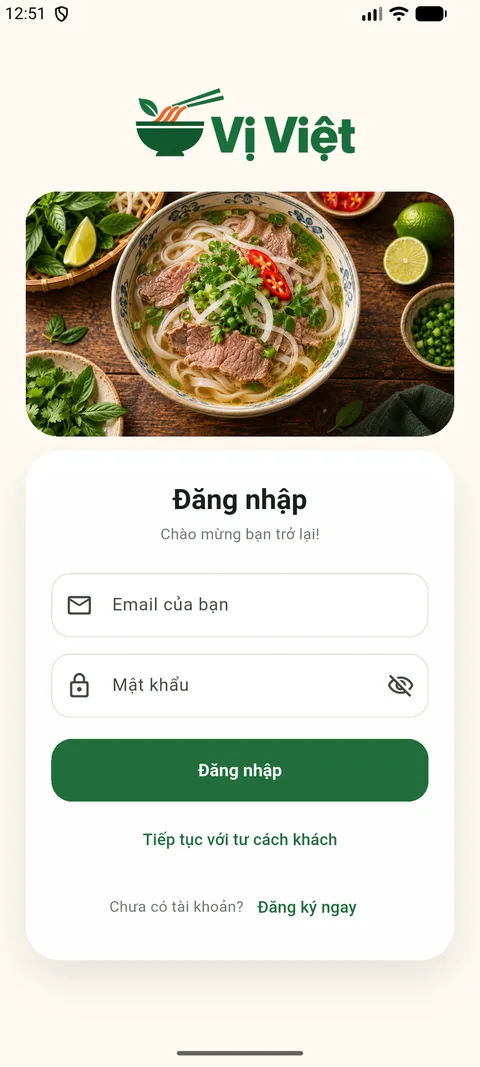
\includegraphics[width=\linewidth,height=.42\textheight,keepaspectratio]{figs/ui/login.png}\\[3pt]
\small Đăng nhập
\end{minipage}\hfill
\begin{minipage}[t]{0.31\textwidth}\centering
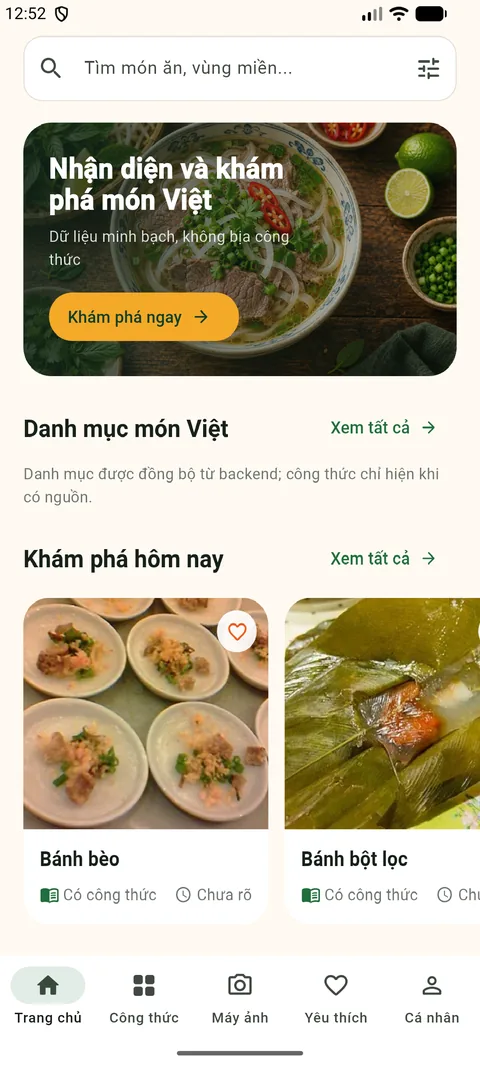
\includegraphics[width=\linewidth,height=.42\textheight,keepaspectratio]{figs/ui/home.png}\\[3pt]
\small Trang chủ
\end{minipage}\hfill
\begin{minipage}[t]{0.31\textwidth}\centering
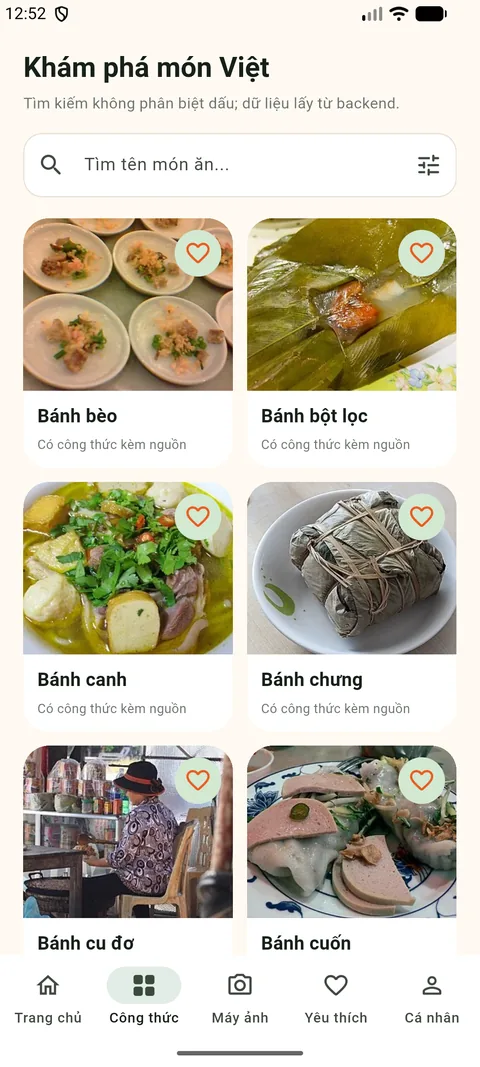
\includegraphics[width=\linewidth,height=.42\textheight,keepaspectratio]{figs/ui/recipes.png}\\[3pt]
\small Danh mục công thức
\end{minipage}
\caption{Các màn hình đăng nhập, trang chủ và danh mục.}
\label{fig:ui-auth-home}
\end{figure}

Hình~\ref{fig:ui-ai-recipe} minh họa luồng nhận diện Phở và khu vực nguồn--bản
quyền. Ảnh kết quả chỉ hiển thị một dự đoán cao nhất theo định hướng tối giản.

\begin{figure}[htbp]
\centering
\begin{minipage}[t]{0.31\textwidth}\centering
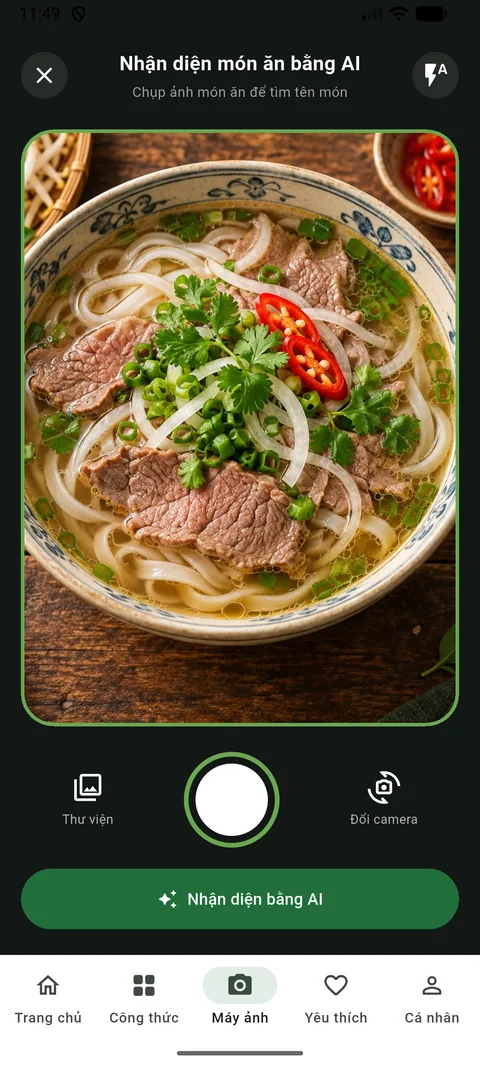
\includegraphics[width=\linewidth,height=.42\textheight,keepaspectratio]{figs/ui/ai-camera-pho.png}\\[3pt]
\small Chọn ảnh Phở
\end{minipage}\hfill
\begin{minipage}[t]{0.31\textwidth}\centering
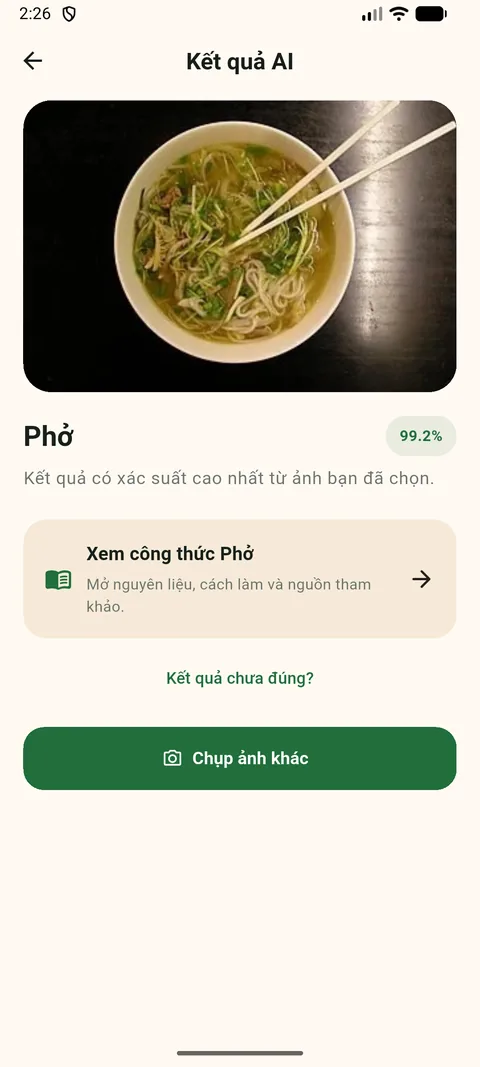
\includegraphics[width=\linewidth,height=.42\textheight,keepaspectratio]{figs/ui/ai-result-pho.png}\\[3pt]
\small Kết quả Top~1
\end{minipage}\hfill
\begin{minipage}[t]{0.31\textwidth}\centering
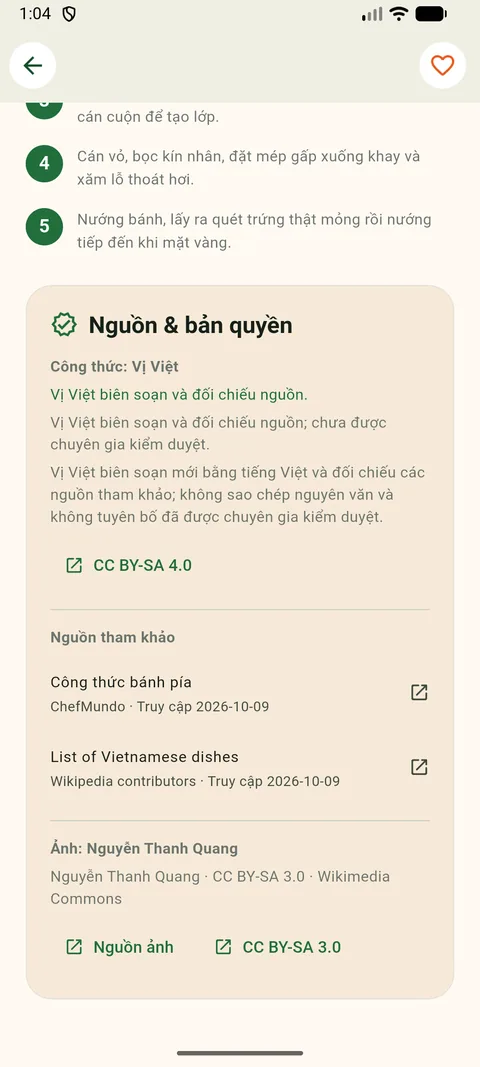
\includegraphics[width=\linewidth,height=.42\textheight,keepaspectratio]{figs/ui/recipe-license.png}\\[3pt]
\small Nguồn và bản quyền
\end{minipage}
\caption{Luồng nhận diện và xem công thức có nguồn.}
\label{fig:ui-ai-recipe}
\end{figure}

\section{Chiến lược kiểm thử}

Backend có 24 test case bao phủ bảo mật, database, model loader, xử lý ảnh,
API và luồng MVP. Flutter có 21 test/widget test cho parse model, refresh
token, optimistic update, màn kết quả, metadata công thức, hồ sơ và điều
hướng đăng ký. Ngoài tự động, audit dữ liệu kiểm tra 38 món, ảnh, metadata và
toàn vẹn catalog. APK debug và hai luồng danh mục--chi tiết, nhận diện--công
thức được dùng để nghiệm thu trên Emulator.

\begin{table}[htbp]
\centering
\caption{Nhóm kiểm thử của hệ thống.}
\label{tab:test-groups}
\begin{tabularx}{\textwidth}{>{\bfseries}p{3.2cm} X}
\toprule
Nhóm & Nội dung \\
\midrule
Backend unit/API & Xác thực, rate limit, ảnh lỗi, CRUD, predict và serializer \\
Flutter & State, parse JSON, điều hướng, dialog, màn kết quả và responsive \\
Data audit & 38 công thức, ảnh, nguồn, thời gian, rollback và idempotency \\
Build & Phân tích tĩnh, test, APK debug và cấu hình Android Studio \\
Emulator & Đăng nhập, tìm kiếm, camera/thư viện, Top~1 và mở công thức \\
\bottomrule
\end{tabularx}
\end{table}

\chapter{Kết quả và đánh giá}
\label{ch:ketqua}

\begin{muctieu}
Chương này đối chiếu mục tiêu, trình bày audit dữ liệu, đánh giá model trên
tập Test sạch và phân tích những hạn chế của sản phẩm.
\end{muctieu}

\newcommand{\EvalTotal}{5.014}
\newcommand{\EvalCorrect}{4.690}
\newcommand{\EvalAccuracy}{93,54\%}
\newcommand{\EvalMacroPrecision}{94,00\%}
\newcommand{\EvalMacroRecall}{93,41\%}
\newcommand{\EvalMacroFOne}{93,68\%}
\newcommand{\EvalMeanConfidence}{93,30\%}
\newcommand{\EvalMeanMs}{1410,0}
\newcommand{\EvalPPercentileMs}{1406,8}


\section{Mức độ hoàn thành mục tiêu}

Ứng dụng đã hoàn thiện luồng Flutter--FastAPI, nhận diện ảnh bằng model 38
nhãn, tìm kiếm và hiển thị 38 công thức có nguồn. Các chức năng đăng ký,
đăng nhập, chế độ khách, yêu thích, lịch sử, phản hồi và sửa tên được tích
hợp. Backend có migration, audit, importer và tài liệu OpenAPI. Như vậy năm
nhóm mục tiêu sản phẩm ở Chương~\ref{ch:modau} đã được hiện thực; phạm vi
production nhiều người dùng vẫn là hướng phát triển.

\section{Kết quả dữ liệu công thức}

\begin{table}[htbp]
\centering
\caption{Thống kê kho công thức sau audit.}
\label{tab:recipe-audit}
\begin{tabular}{>{\bfseries}l r}
\toprule
Thuộc tính & Kết quả \\
\midrule
Món đã xuất bản & 38/38 \\
Ảnh có metadata đầy đủ & 38/38 \\
Nguyên liệu & 348 \\
Bước thực hiện & 205 \\
Nguồn tham khảo & 85 \\
Công thức dịch nguồn mở & 8 \\
Công thức biên soạn đối chiếu & 30 \\
\bottomrule
\end{tabular}
\end{table}

Audit xác nhận mỗi món có thời gian sơ chế, nấu, tổng thời gian, khẩu phần,
ít nhất một nguyên liệu và một bước. Ảnh local giải mã được và metadata khớp
manifest. Việc tách catalog nguồn mở với catalog biên soạn giúp hiển thị đúng
nguồn gốc nội dung và phạm vi giấy phép.

\section{Audit và làm sạch 30VNFoods}

Dataset gốc có 25.136 ảnh JPG thuộc 30 lớp: 17.581 Train, 2.515 Validate và
5.040 Test. Tất cả ảnh đều được Pillow đọc thành công. Audit SHA-256 phát
hiện 63 nhóm trùng, 40 nhóm đi qua nhiều split và 38 nhóm có cùng ảnh nhưng
khác nhãn. Chính sách làm sạch giữ một bản cho nhóm trùng cùng nhãn, ưu tiên
Test rồi Validate và Train; nhóm mâu thuẫn nhãn bị loại hoàn toàn.

Manifest sạch còn 25.032 ảnh: 17.515 Train, 2.503 Validate và 5.014 Test như
Hình~\ref{fig:dataset-splits}. Dữ liệu raw không bị sửa.

\begin{figure}[htbp]
\centering
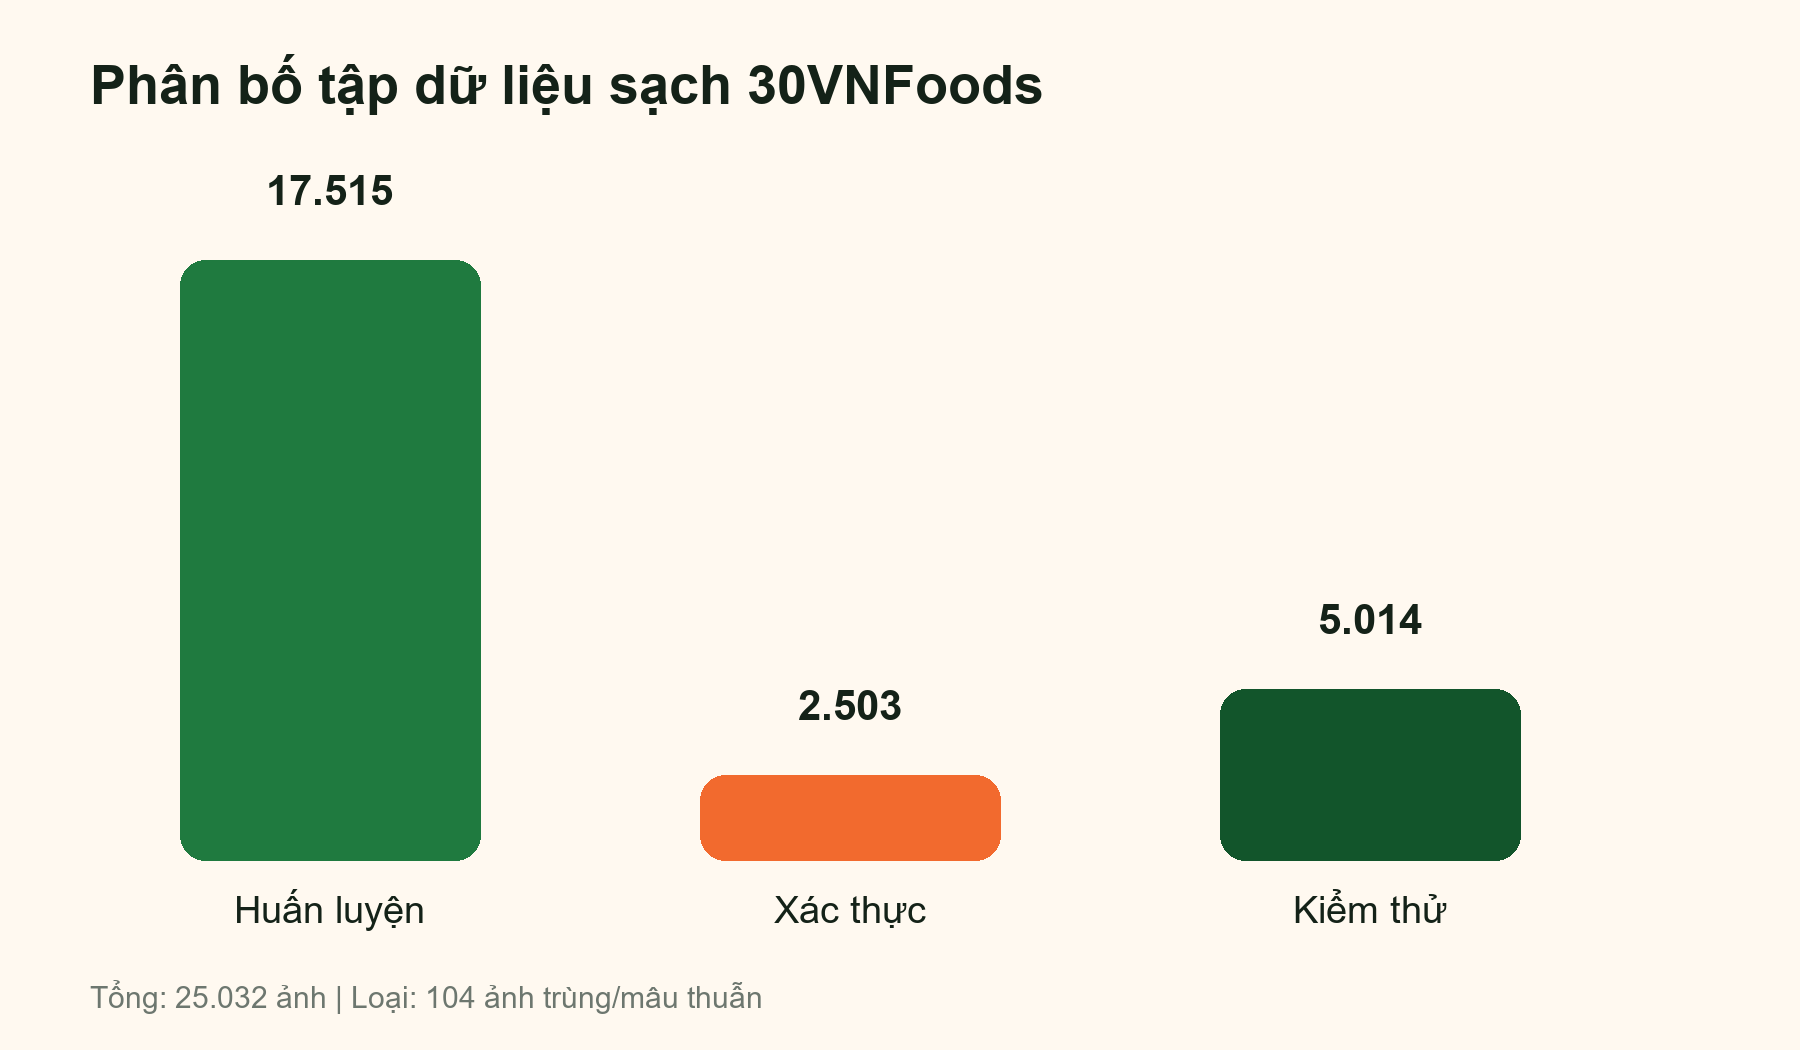
\includegraphics[width=0.88\textwidth]{figs/charts/dataset-splits.png}
\caption{Phân bố các split sau khi loại ảnh trùng và mâu thuẫn.}
\label{fig:dataset-splits}
\end{figure}

Số ảnh giữa các lớp không hoàn toàn cân bằng. Hình~\ref{fig:dataset-classes}
cho thấy Bún bò Huế, Bánh mì và Bánh xèo có nhiều mẫu hơn một số lớp như Bánh
pía hoặc Bánh chưng. Vì vậy báo cáo sử dụng thêm macro F1 thay vì chỉ đọc
accuracy.

\clearpage
\thispagestyle{dau}
\vspace*{\fill}
\begin{center}
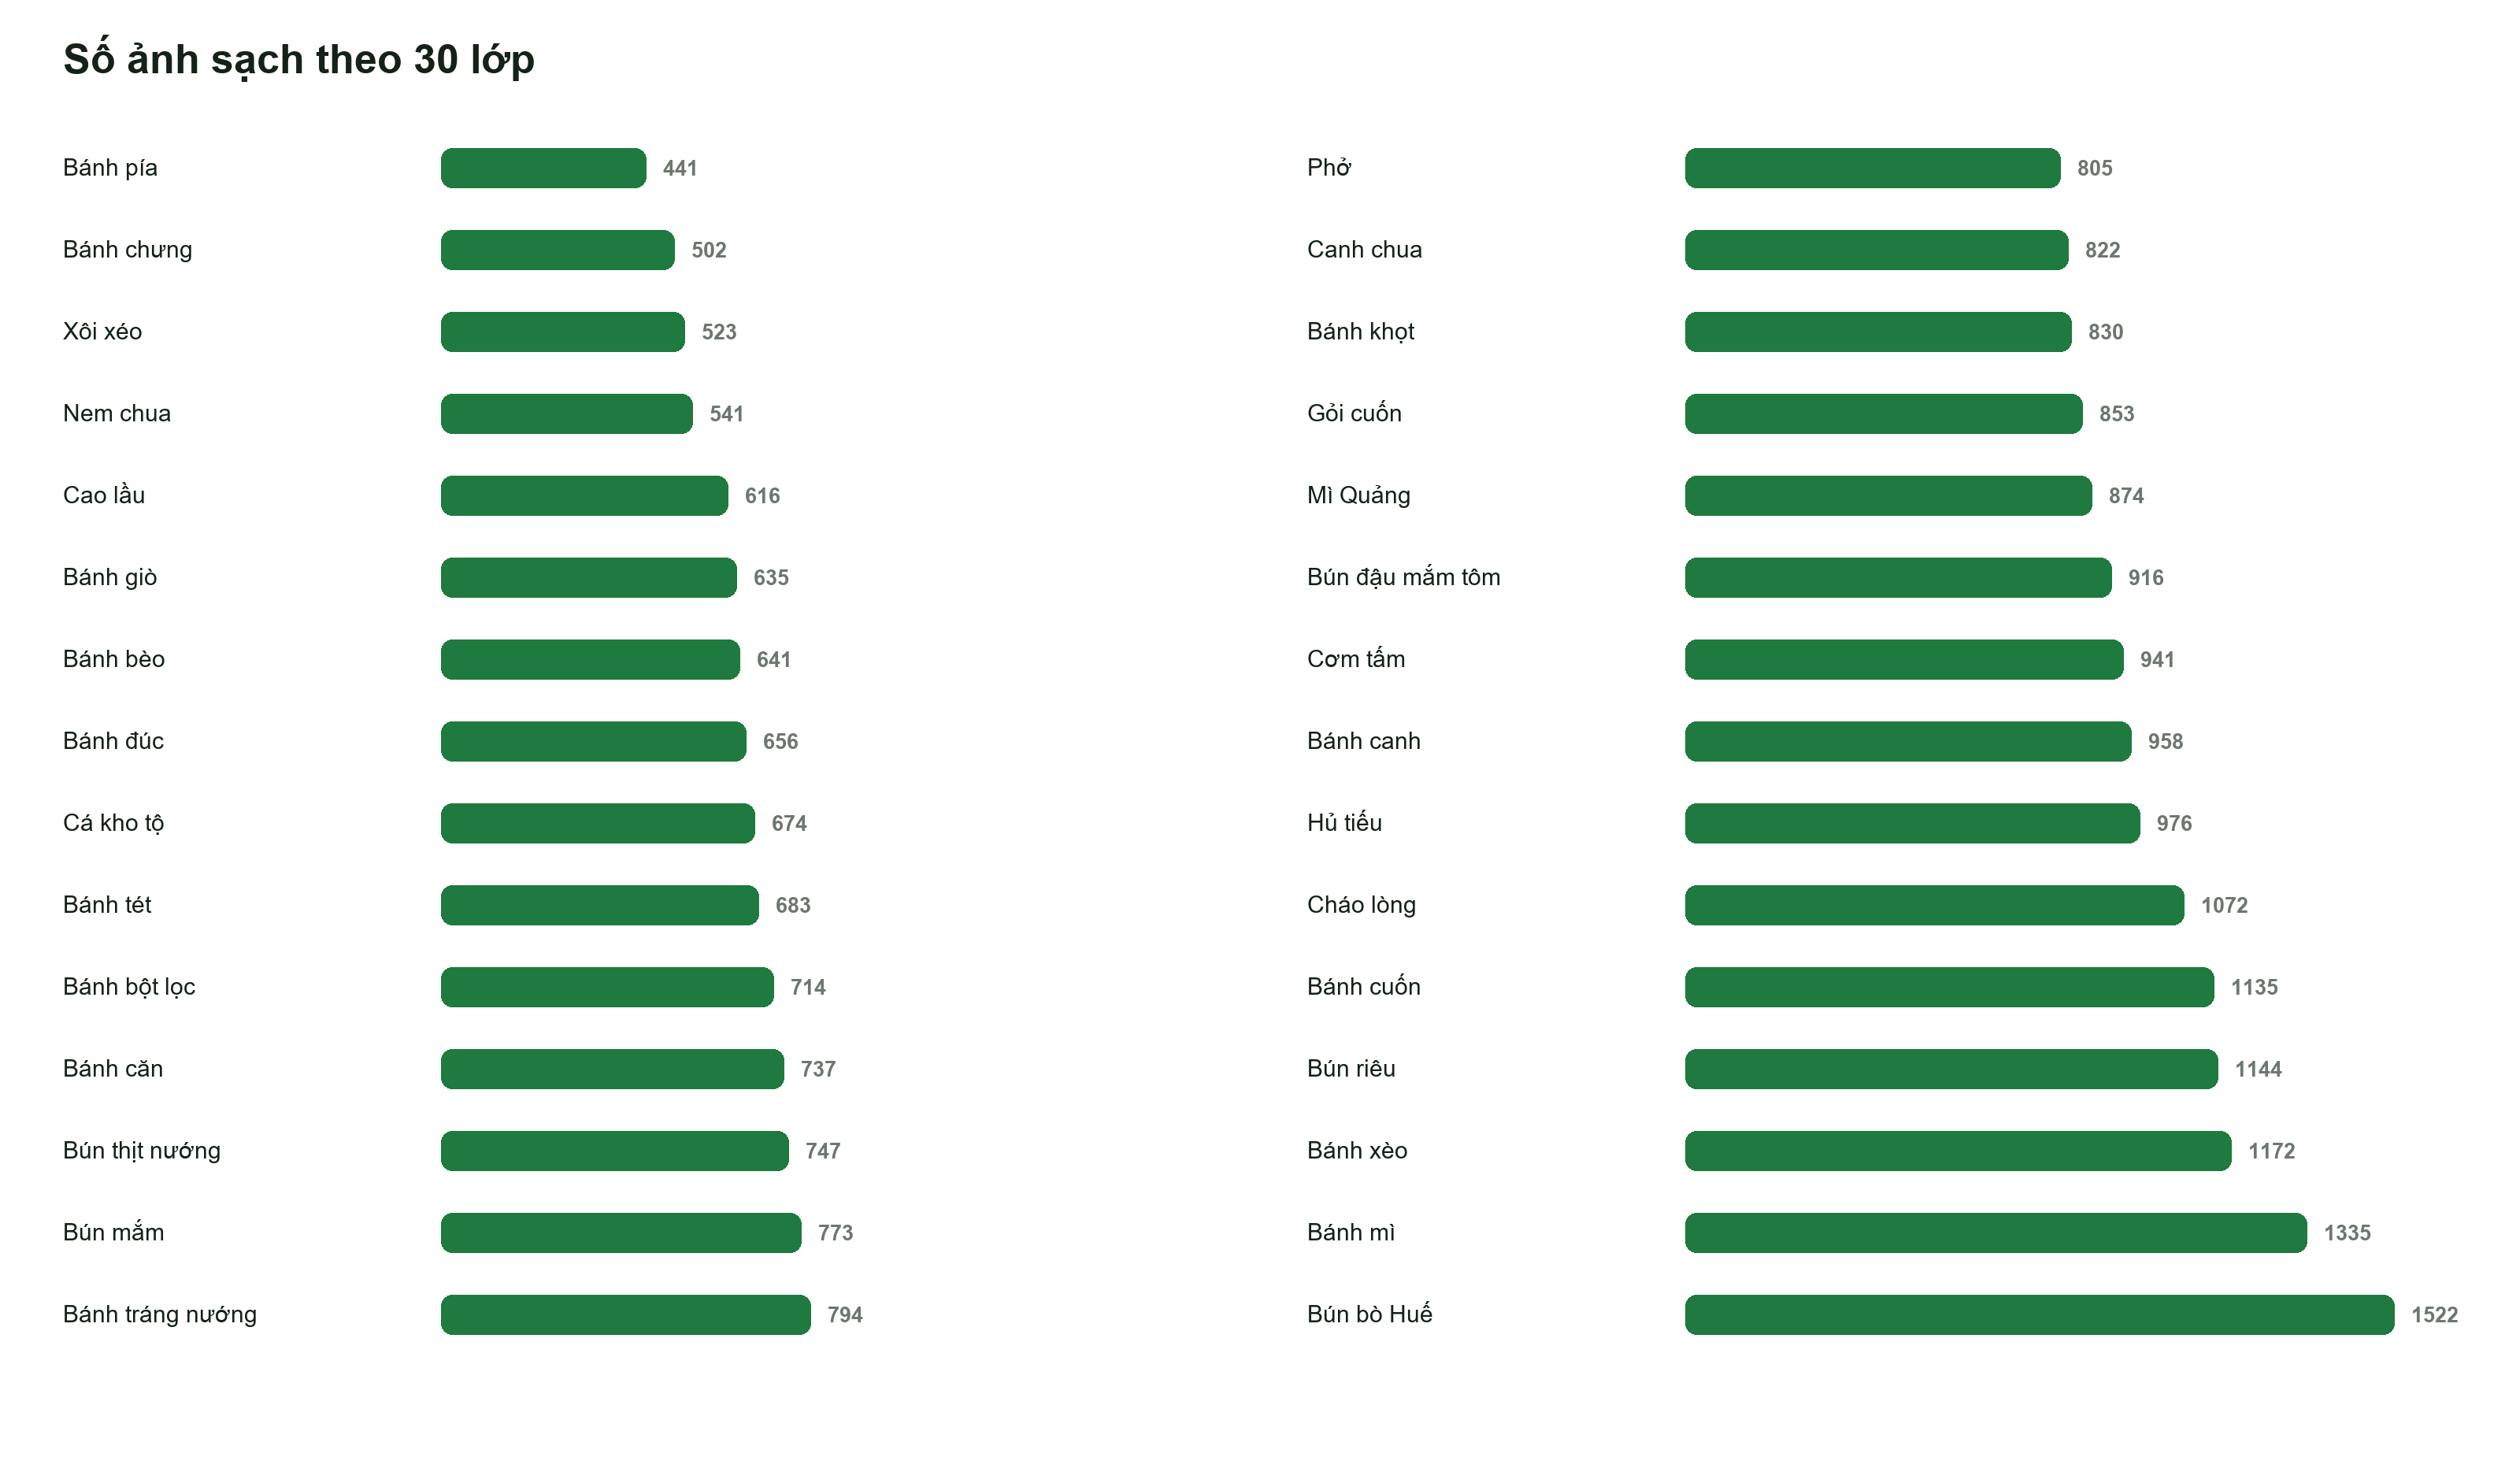
\includegraphics[width=\textwidth]{figs/charts/dataset-classes.png}
\dauFigureCaption{Số ảnh sạch theo từng lớp trong toàn bộ ba split.}{fig:dataset-classes}
\end{center}
\vspace*{\fill}
\clearpage

\section{Kết quả đánh giá model}

Model được chạy trên toàn bộ \EvalTotal{} ảnh của manifest Test sạch. Nhãn
dataset được chuẩn hóa bằng cùng module alias với backend. Một dự đoán chỉ
được tính đúng khi tên chuẩn Top~1 trùng ground truth. Các dự đoán rơi vào
tám lớp ngoài phạm vi 30VNFoods vẫn được tính là sai.

\begin{table}[htbp]
\centering
\caption{Kết quả đánh giá trên tập Test sạch.}
\label{tab:model-metrics}
\begin{tabular}{>{\bfseries}l r}
\toprule
Độ đo & Giá trị \\
\midrule
Số ảnh đánh giá & \EvalTotal \\
Số dự đoán đúng & \EvalCorrect \\
Accuracy Top~1 & \EvalAccuracy \\
Macro Precision & \EvalMacroPrecision \\
Macro Recall & \EvalMacroRecall \\
Macro F1 & \EvalMacroFOne \\
Confidence trung bình & \EvalMeanConfidence \\
Thời gian trung bình/ảnh & \EvalMeanMs{} ms \\
P95 thời gian/ảnh & \EvalPPercentileMs{} ms \\
\bottomrule
\end{tabular}
\end{table}

Các con số trong Bảng~\ref{tab:model-metrics} là kết quả chạy tại máy thử
nghiệm, không phải số liệu do model card công bố. Thời gian/ảnh được chia đều
theo batch và phụ thuộc thiết bị, backend, batch size và trạng thái bộ nhớ.

\IfFileExists{figs/charts/per-class-metrics.png}{
\clearpage
\thispagestyle{dau}
\vspace*{\fill}
\begin{center}
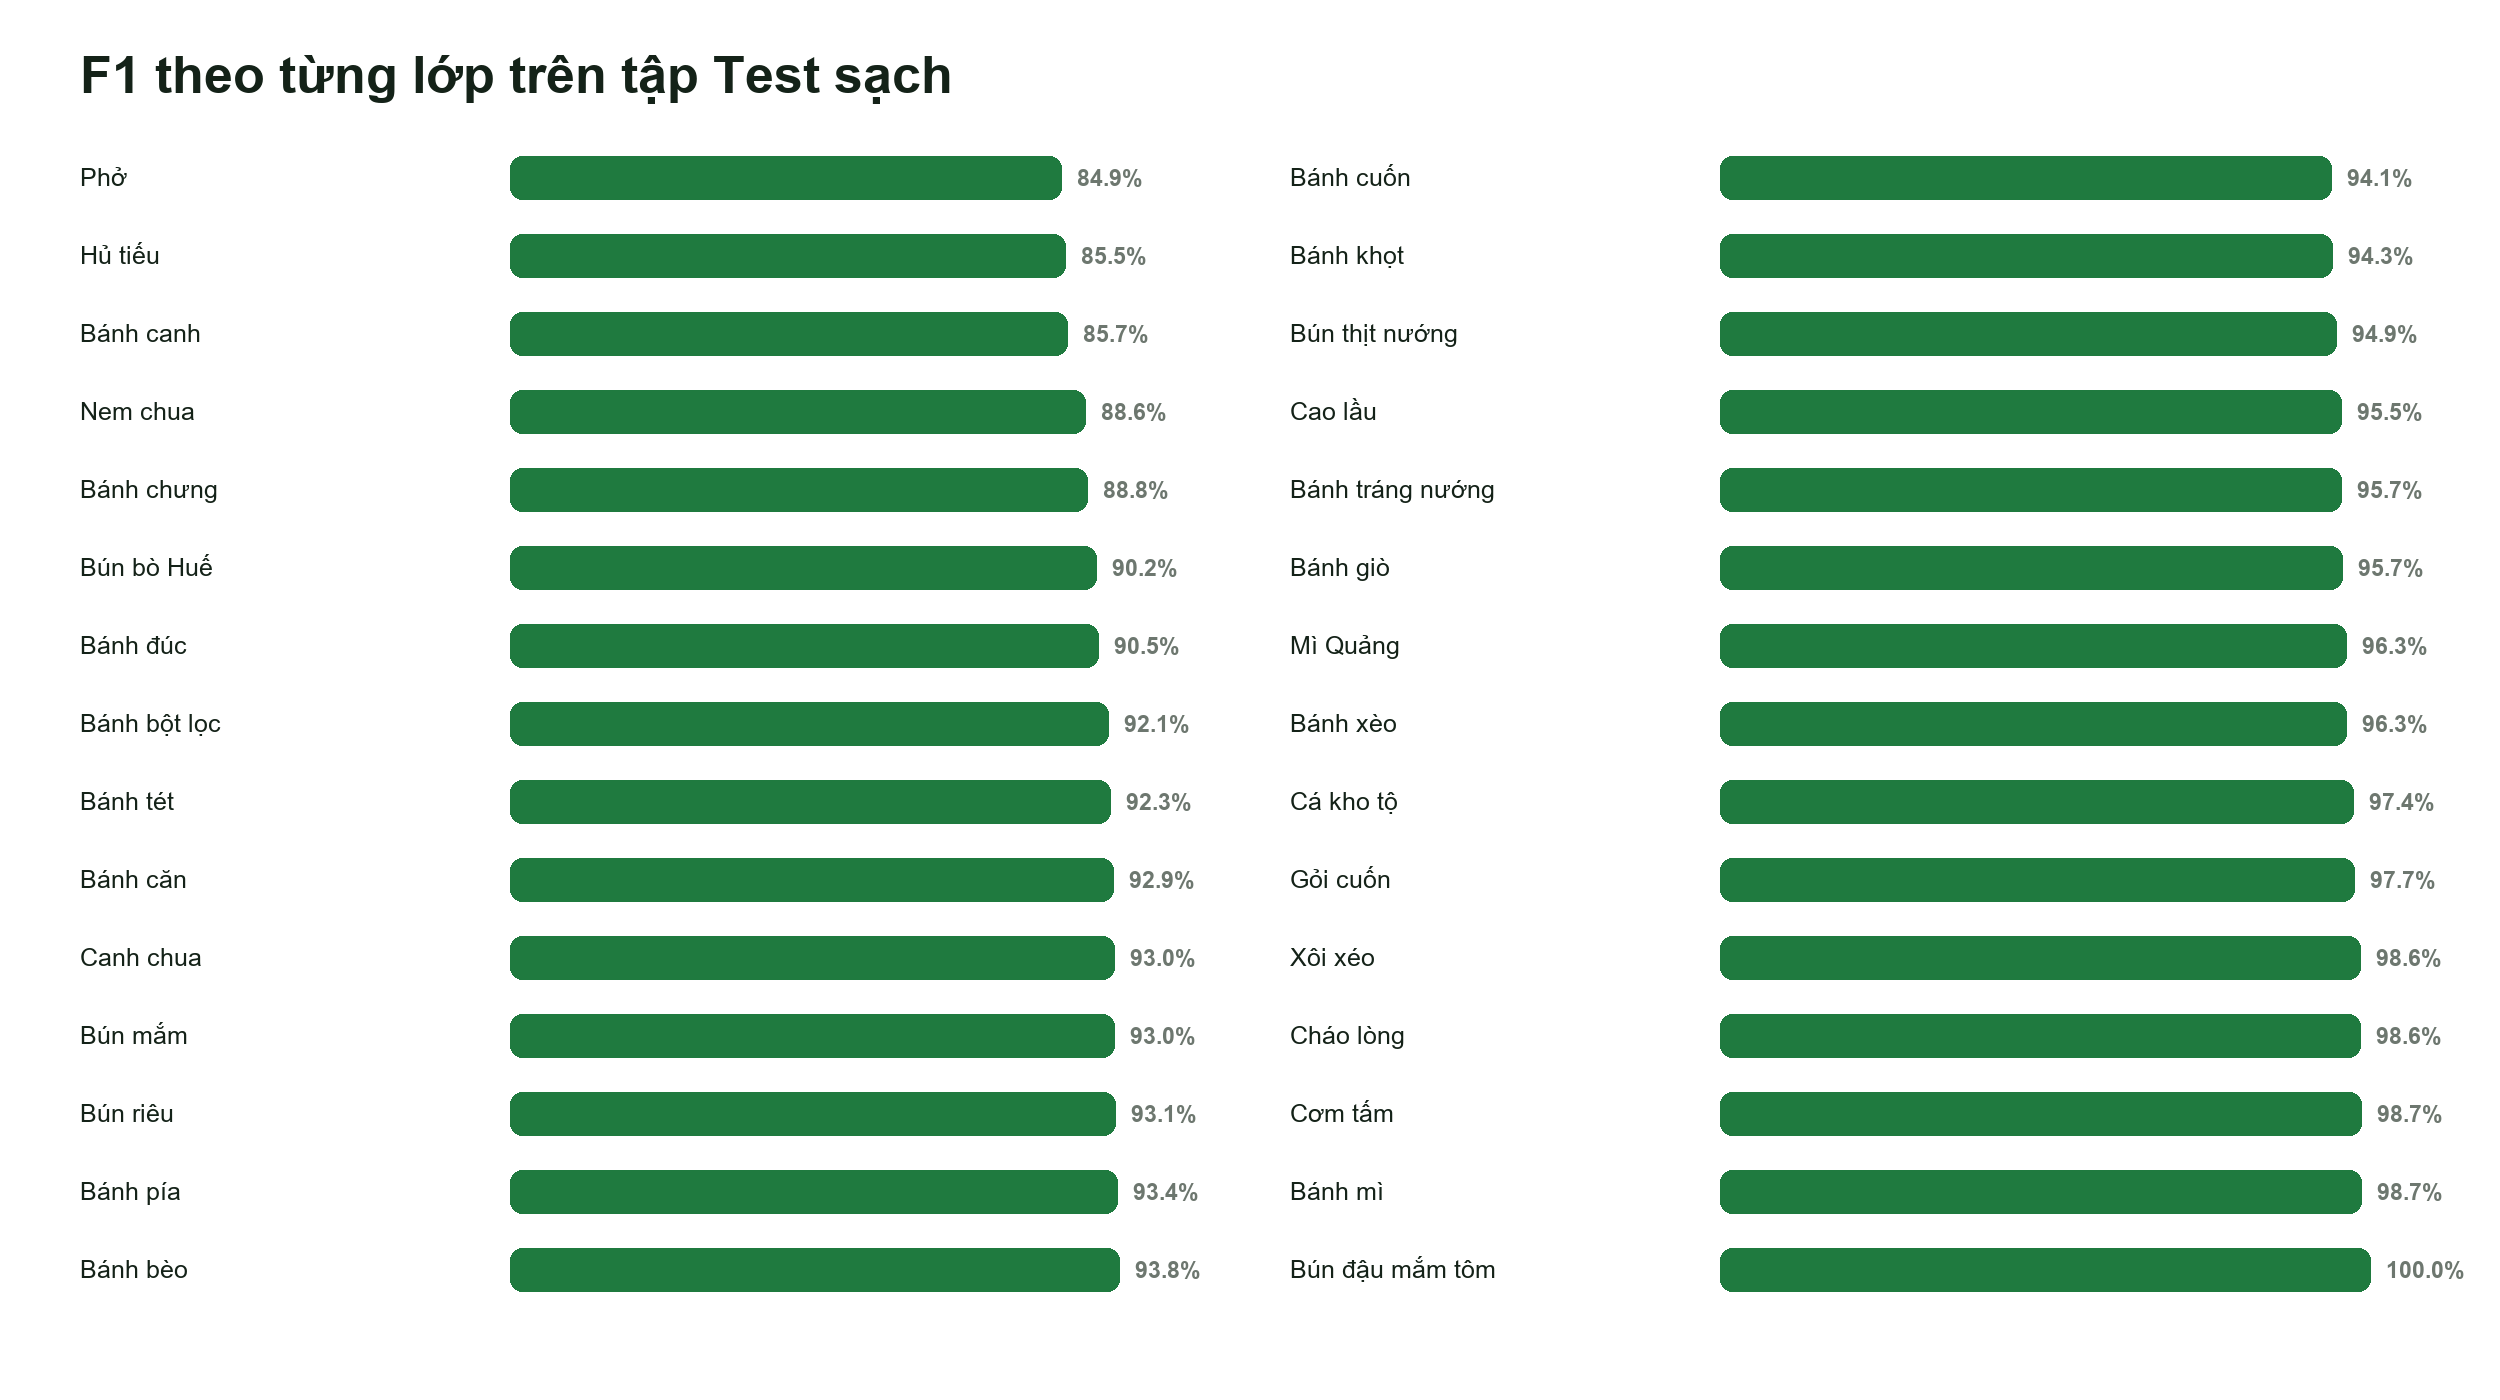
\includegraphics[width=\textwidth]{figs/charts/per-class-metrics.png}
\dauFigureCaption{F1 theo từng lớp trên tập Test sạch.}{fig:per-class-metrics}
\end{center}
\vspace*{\fill}
\clearpage
\thispagestyle{dau}
\vspace*{\fill}
\begin{center}
\IfFileExists{figs/charts/confusion-matrix.png}{%
  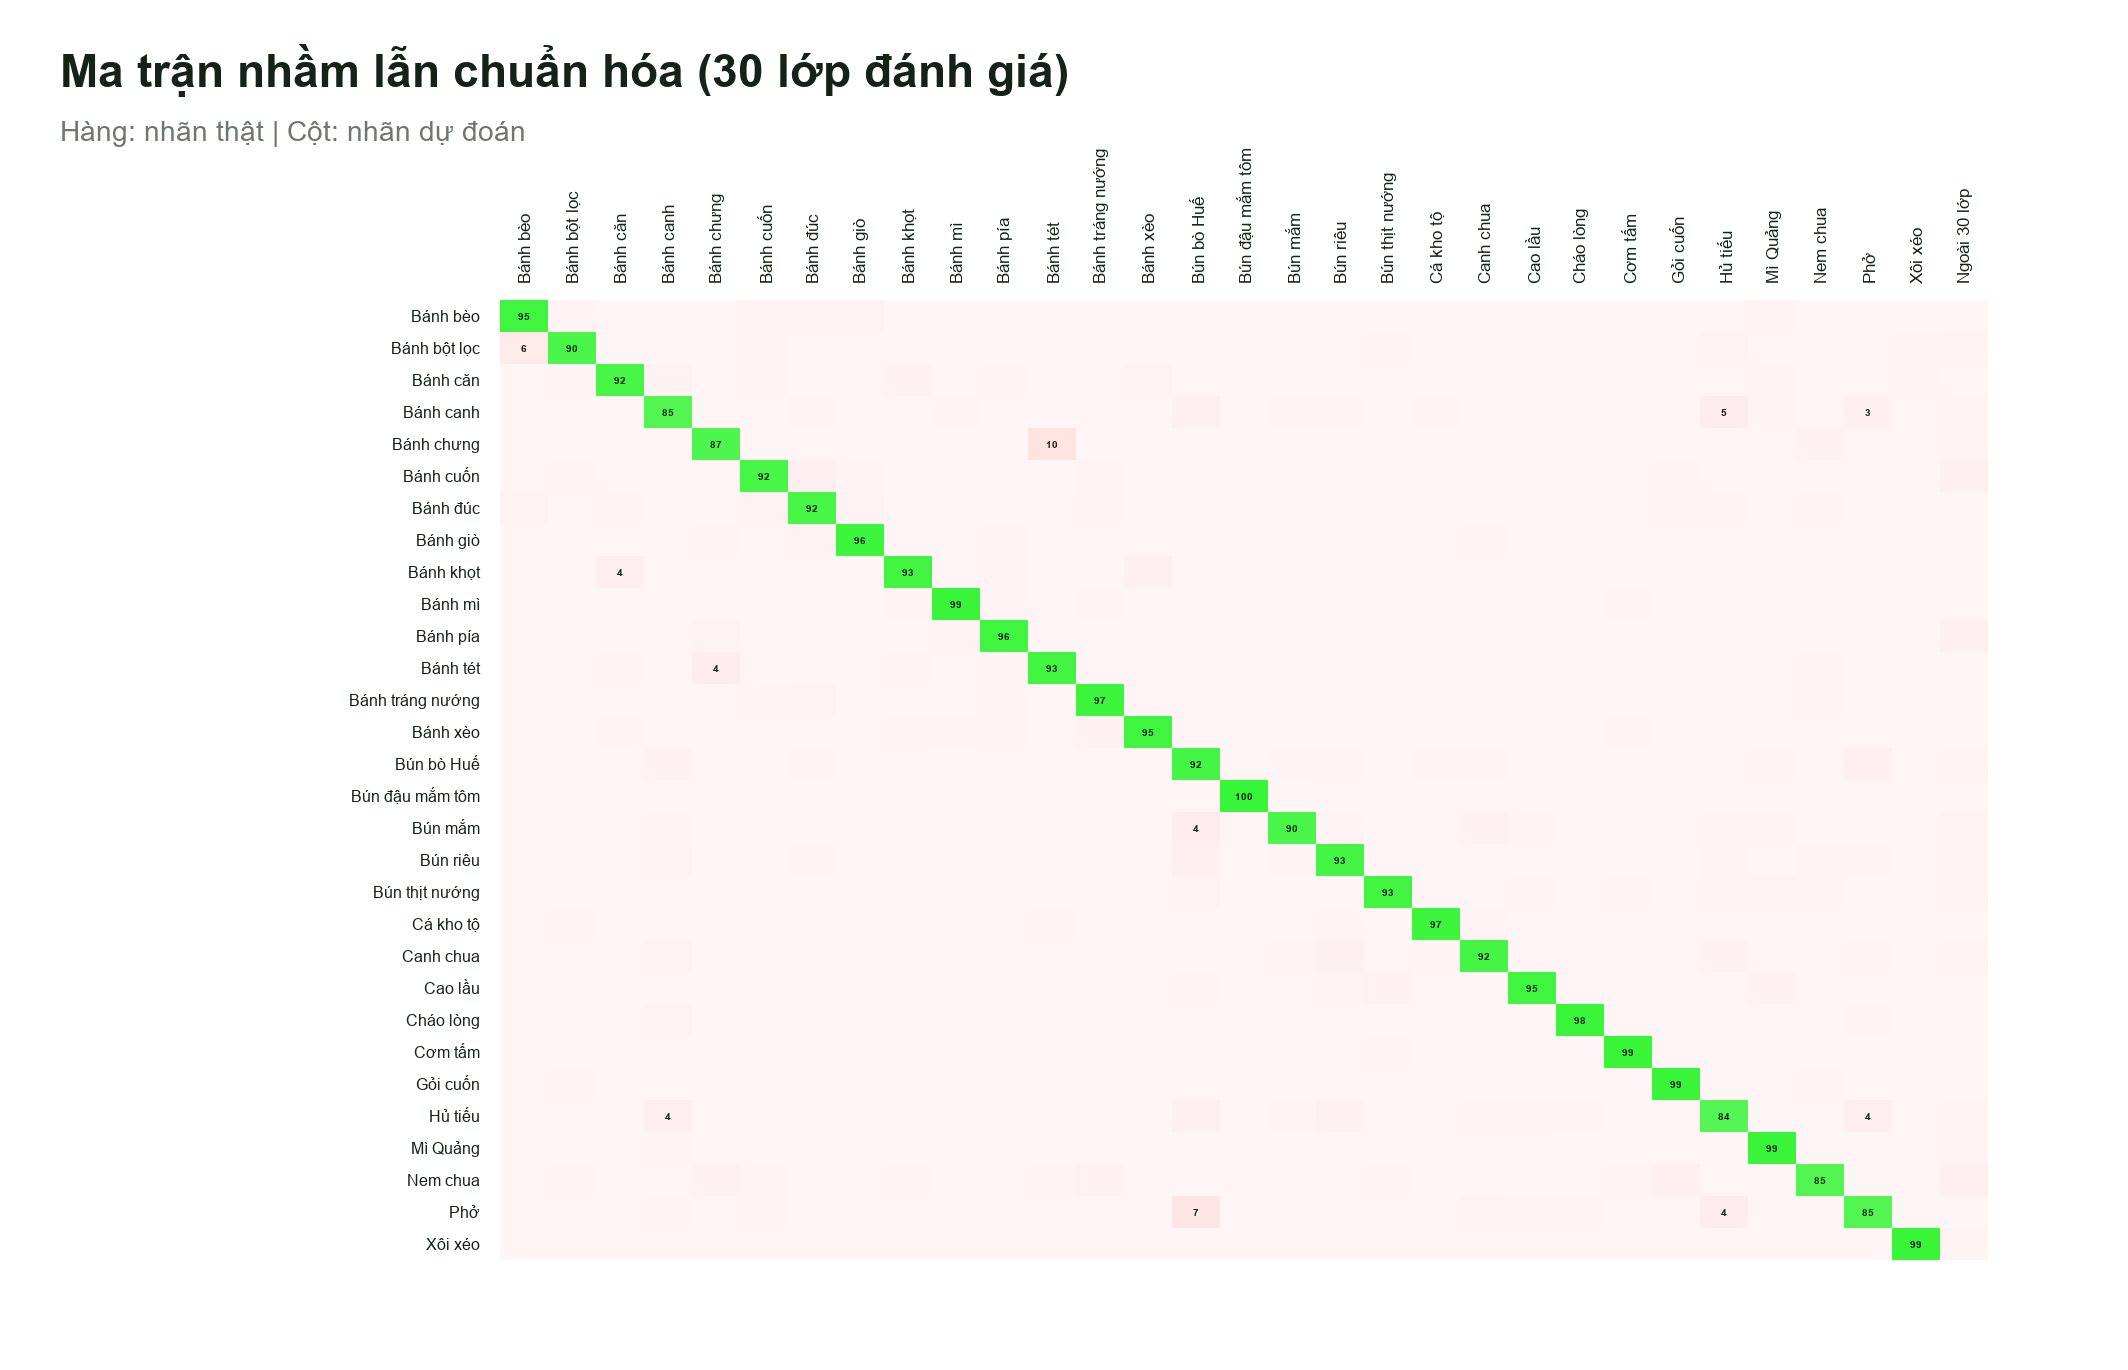
\includegraphics[width=\textwidth,height=0.72\textheight,keepaspectratio]{figs/charts/confusion-matrix.png}
  \dauFigureCaption{Ma trận nhầm lẫn chuẩn hóa; tám nhãn ngoài dataset được gộp thành một cột.}{fig:confusion-matrix}%
}{}
\end{center}
\vspace*{\fill}
\clearpage
}{}

\IfFileExists{evaluation/top-confusions.tex}{\begin{table}[htbp]
\centering
\caption{Các cặp nhầm lẫn xuất hiện nhiều nhất.}
\label{tab:top-confusions}
\begin{tabular}{>{\bfseries}l l r}
\toprule Nhãn thật & Dự đoán & Số ảnh \\
\midrule
Phở & Bún bò Huế & 12 \\
Bánh chưng & Bánh tét & 10 \\
Bánh canh & Hủ tiếu & 9 \\
Bún bò Huế & Phở & 9 \\
Bánh bột lọc & Bánh bèo & 8 \\
Hủ tiếu & Phở & 7 \\
Hủ tiếu & Bánh canh & 7 \\
Bánh canh & Phở & 6 \\
Bánh cuốn & Bánh đúc & 6 \\
Bánh khọt & Bánh căn & 6 \\
\bottomrule
\end{tabular}
\end{table}
}{}

\section{Kết quả kiểm thử phần mềm}

\IfFileExists{evaluation/test-status.tex}{\begin{table}[htbp]
\centering
\caption{Kết quả kiểm thử và build tại lần nghiệm thu báo cáo.}
\label{tab:test-status}
\begin{tabularx}{\textwidth}{>{\bfseries}p{4.1cm} p{2.3cm} X}
\toprule
Hạng mục & Trạng thái & Kết quả \\
\midrule
Backend pytest & PASS & 24 test, 48 subtest; 2 cảnh báo deprecation; 12,24 giây \\
Flutter analyze & PASS & Không phát hiện issue; 53,4 giây \\
Flutter test & PASS & 21/21 test; khoảng 5 giây \\
Audit công thức & PASS & 38 món, 38 ảnh, metadata đầy đủ, không có lỗi \\
Build APK debug & PASS & Sinh \code{mobile/build/}\\\code{app/outputs/}\\\code{flutter-apk/}\\\code{app-debug.apk} \\
Android Emulator & CHƯA THỬ LẠI & Có ảnh nghiệm thu luồng camera, Top~1 và mở công thức; chưa chạy lại thao tác tương tác trong phiên tạo báo cáo \\
\bottomrule
\end{tabularx}
\end{table}

Backend test phát sinh hai cảnh báo không làm test thất bại: TestClient của
Starlette sẽ chuyển sang \code{httpx2}, và cấu hình Alembic chưa khai báo
\code{path\_separator}. APK build có cảnh báo phiên bản SDK XML giữa Android
Studio và command-line tools nhưng Gradle vẫn kết thúc với mã thoát 0.
}{
\begin{luuy}
Kết quả kiểm thử tự động chưa được ghi nhận bằng mã thoát rõ ràng. Không được
tuyên bố PASS trước khi chạy lại và lưu log.
\end{luuy}}

Audit công thức đã chạy thành công và trả \code{ok=true}, 38 món published,
38 ảnh và 38 bản ghi metadata hoàn chỉnh. Kiểm thử phần mềm được chạy tuần
tự để tránh xung đột cache; trạng thái trong bảng được lấy từ log cùng lần
nghiệm thu báo cáo.

\section{Bàn luận}

Kết quả cần được đọc trong bối cảnh 30VNFoods chỉ có 30/38 nhãn. Accuracy và
macro F1 đo khả năng nhận diện trên phần giao nhau, không chứng minh hiệu
năng với Bánh cu đơ, Nem nướng, Bánh mì cay, Cơm cháy, Bò bía, Bánh đậu xanh,
Bánh đa cua và Bún cá. Những lớp có hình dạng hoặc thành phần gần nhau dễ gây
nhầm lẫn; ma trận nhầm lẫn giúp xác định cặp cần bổ sung dữ liệu.

Điểm mạnh của hệ thống không chỉ nằm ở model. Sau khi có nhãn, backend phải
ánh xạ đúng tên có dấu, trả đúng món và không tự tạo công thức khi ánh xạ
thất bại. Việc lưu Top~3 ở backend nhưng chỉ hiển thị Top~1 giúp giữ dữ liệu
phục vụ phân tích mà không làm giao diện phức tạp.

\section{Hạn chế}

\begin{itemize}
  \item Bộ đánh giá không bao phủ tám nhãn model; chưa có tập test độc lập
        đồng nhất cho đủ 38 món.
  \item Model ViT-L/16 khoảng 1,21~GB, tốn RAM và có thể chậm khi suy luận CPU.
  \item Model card cho biết dữ liệu huấn luyện có phần tự thu thập; báo cáo
        không thể audit toàn bộ dữ liệu huấn luyện gốc của tác giả model.
  \item SQLite và rate limiter trong bộ nhớ phù hợp demo đơn máy, chưa phù
        hợp nhiều API instance ghi đồng thời.
  \item Chưa có deployment công khai, CI/CD hoặc kiểm thử tải dài hạn.
  \item Công thức có nguồn đối chiếu nhưng chưa được chuyên gia dinh dưỡng
        hoặc đầu bếp kiểm duyệt.
\end{itemize}

\chapter{Kết luận và hướng phát triển}
\label{ch:ketluan}

\begin{muctieu}
Chương này tổng kết kết quả, bài học rút ra và các hướng phát triển khả thi
từ những hạn chế đã phân tích.
\end{muctieu}

\section{Kết luận}

Đồ án đã xây dựng một hệ thống mobile hoàn chỉnh cho khám phá công thức và
nhận diện món Việt. Ứng dụng Flutter kết nối FastAPI, database SQLite và model
ViT-L/16; nhãn model được chuẩn hóa rồi ánh xạ tới 38 món có công thức, ảnh,
nguồn và giấy phép. Ngoài luồng AI, hệ thống hỗ trợ tìm kiếm, lọc, tài khoản,
yêu thích, lịch sử và phản hồi.

Đóng góp quan trọng của đồ án là kết nối ba loại dữ liệu vốn tách rời: ảnh
nhận diện, nhãn model và catalog công thức. Quy trình audit giúp tránh sử
dụng ảnh train làm ảnh giao diện, tránh công thức không rõ nguồn và tránh
tuyên bố hiệu năng model dựa trên một mẫu quá nhỏ. Đánh giá đầy đủ được thực
hiện trên 5.014 ảnh Test sạch thuộc 30 lớp có thể đối chiếu.

\section{Bài học rút ra}

Chất lượng dữ liệu ảnh ảnh hưởng trực tiếp tới độ tin cậy của đánh giá. Nếu
không loại ảnh trùng qua split, kết quả có thể lạc quan giả tạo. Với dữ liệu
công thức, có nội dung chưa đủ; mỗi ảnh và công thức còn cần metadata nguồn,
giấy phép và dấu vết thay đổi. Vì vậy phần audit và importer chiếm vai trò
không nhỏ hơn việc tích hợp model.

\begin{samepage}
Một model mạnh không tự tạo thành sản phẩm tốt. Hệ thống phải xử lý ảnh hỏng,
model chưa sẵn sàng, mất mạng, token hết hạn, nhãn không ánh xạ được và recipe
không hợp lệ. Tách UI, service, state, router và repository giúp từng trường
hợp có thể kiểm thử độc lập. Nếu thực hiện lại, việc xây dựng tiêu chí dữ liệu
và bộ test độc lập sẽ được ưu tiên ngay từ đầu.
\end{samepage}

Trí tuệ nhân tạo trong hệ thống đóng vai trò gợi ý, không phải kết luận tuyệt
đối. Confidence phải được trình bày minh bạch và người dùng cần có cơ chế gửi
phản hồi. Tương tự, công cụ AI hỗ trợ phát triển phải được kiểm chứng bằng mã
nguồn, test và nguồn tham khảo trước khi đưa vào báo cáo.

\section{Hướng phát triển}

\begin{itemize}
  \item \textbf{Đủ dữ liệu cho 38 nhãn:} xây dựng tập test có giấy phép và
        quy trình gán nhãn cho tám món còn thiếu, từ đó đánh giá đúng toàn bộ
        phạm vi production.
  \item \textbf{Fine-tune có kiểm soát:} huấn luyện candidate trên manifest
        sạch, so sánh trên test độc lập và chỉ thay production model khi có
        cải thiện được chứng minh.
  \item \textbf{Tối ưu suy luận:} thử nghiệm model nhỏ hơn, quantization,
        ONNX/TFLite hoặc GPU server để giảm thời gian và dung lượng.
  \item \textbf{Hạ tầng production:} chuyển sang PostgreSQL, rate limiter
        dùng kho chia sẻ, reverse proxy, HTTPS, log tập trung và monitoring.
  \item \textbf{Vòng phản hồi:} tổng hợp nhãn người dùng xác nhận thành hàng
        đợi kiểm duyệt, không đưa thẳng dữ liệu chưa kiểm chứng vào train.
  \item \textbf{Mở rộng nội dung:} bổ sung dinh dưỡng, dị ứng và biến thể
        vùng miền khi có nguồn chuyên môn phù hợp.
\end{itemize}


\backmatter
\cleardoublepage
\phantomsection
\addcontentsline{toc}{chapter}{Tài liệu tham khảo}
\bibliographystyle{plain}
\bibliography{refs}
\chapter{Phụ lục}
\markboth{Phụ lục}{}

\section*{A. Hướng dẫn cài đặt và chạy chương trình}
\phantomsection
\addcontentsline{toc}{section}{A. Hướng dẫn cài đặt và chạy chương trình}

Từ thư mục gốc dự án trên Windows, thiết lập backend bằng các lệnh sau:

\begin{lstlisting}[language=bash, caption={Thiết lập và chạy backend.}]
setup_backend.bat
run_backend.bat
\end{lstlisting}

Script tạo môi trường Python, cài dependency và tải model khi chưa có. Sau
khi API báo \code{/health} thành công, mở thư mục gốc bằng Android Studio,
chọn cấu hình Flutter trỏ tới \code{mobile/lib/main.dart}, mở Android Emulator
và nhấn \code{Shift+F10}. Backend không được tự khởi động từ Gradle.

Kiểm thử thủ công API:
\begin{lstlisting}[language=bash, caption={Kiểm tra health và nhận diện.}]
curl http://127.0.0.1:8000/health
curl -F "image=@food.jpg" http://127.0.0.1:8000/predict
\end{lstlisting}

\section*{B. Danh sách API}
\phantomsection
\addcontentsline{toc}{section}{B. Danh sách API}

\begin{longtable}{p{3.0cm}p{5.2cm}p{5.9cm}}
\caption{Các endpoint chính của backend.}\label{tab:api-list}\\
\toprule Method & Endpoint & Mục đích \\
\midrule \endfirsthead
\toprule Method & Endpoint & Mục đích \\
\midrule \endhead
GET & /health & Kiểm tra API sẵn sàng \\
POST & /auth/register & Tạo tài khoản \\
POST & /auth/login & Đăng nhập \\
POST & /auth/refresh & Xoay vòng token \\
POST & /auth/logout & Thu hồi refresh session \\
GET/PATCH & /users/me & Đọc hoặc đổi họ tên \\
GET & /dishes & Tìm kiếm, lọc và phân trang món \\
GET & /dishes/\{slug\} & Chi tiết món và công thức \\
GET/POST & /favorites & Đọc hoặc thêm yêu thích \\
DELETE & /favorites/\{slug\} & Bỏ yêu thích \\
GET/DELETE & /history & Đọc hoặc xóa lịch sử \\
DELETE & /history/\{id\} & Xóa một lịch sử \\
POST & /predictions/\{id\}/feedback & Gửi nhãn đúng \\
POST & /predict & Nhận diện ảnh món ăn \\
\bottomrule
\end{longtable}

\section*{C. Danh sách 38 món}
\phantomsection
\addcontentsline{toc}{section}{C. Danh sách 38 món}

\begin{enumerate}
\item Bánh cuốn \item Mì Quảng \item Bánh tráng nướng \item Gỏi cuốn
\item Bánh giò \item Bún mắm \item Canh chua \item Nem chua
\item Bún riêu \item Bánh đúc \item Bánh pía \item Bánh canh
\item Bánh khọt \item Bánh bột lọc \item Bánh căn \item Bún thịt nướng
\item Bánh chưng \item Bún đậu mắm tôm \item Bánh bèo \item Bánh tét
\item Cao lầu \item Cháo lòng \item Cá kho tộ \item Bún bò Huế
\item Phở \item Xôi xéo \item Bánh mì \item Bánh xèo
\item Cơm tấm \item Hủ tiếu \item Bánh cu đơ \item Nem nướng
\item Bánh mì cay \item Cơm cháy \item Bò bía \item Bánh đậu xanh
\item Bánh đa cua \item Bún cá
\end{enumerate}

\section*{D. Độ đo chi tiết theo lớp}
\phantomsection
\addcontentsline{toc}{section}{D. Độ đo chi tiết theo lớp}

\IfFileExists{evaluation/per-class-table.tex}{\begin{longtable}{>{\bfseries}p{4.1cm}rrrr}
\caption{Độ đo theo từng lớp trên tập Test sạch.}\label{tab:per-class}\\
\toprule Lớp & Support & Precision & Recall & F1 \\
\midrule \endfirsthead
\toprule Lớp & Support & Precision & Recall & F1 \\
\midrule \endhead
Bánh bèo & 128 & 92,42\% & 95,31\% & 93,85\% \\
Bánh bột lọc & 143 & 94,81\% & 89,51\% & 92,09\% \\
Bánh canh & 191 & 86,63\% & 84,82\% & 85,71\% \\
Bánh chưng & 100 & 90,62\% & 87,00\% & 88,78\% \\
Bánh cuốn & 226 & 96,30\% & 92,04\% & 94,12\% \\
Bánh căn & 149 & 93,84\% & 91,95\% & 92,88\% \\
Bánh giò & 128 & 95,35\% & 96,09\% & 95,72\% \\
Bánh khọt & 167 & 95,12\% & 93,41\% & 94,26\% \\
Bánh mì & 268 & 98,88\% & 98,51\% & 98,69\% \\
Bánh pía & 89 & 91,40\% & 95,51\% & 93,41\% \\
Bánh tráng nướng & 159 & 94,48\% & 96,86\% & 95,65\% \\
Bánh tét & 135 & 91,30\% & 93,33\% & 92,31\% \\
Bánh xèo & 235 & 97,39\% & 95,32\% & 96,34\% \\
Bánh đúc & 130 & 89,47\% & 91,54\% & 90,49\% \\
Bún bò Huế & 305 & 88,36\% & 92,13\% & 90,21\% \\
Bún mắm & 155 & 96,53\% & 89,68\% & 92,98\% \\
Bún riêu & 227 & 93,75\% & 92,51\% & 93,13\% \\
Bún thịt nướng & 150 & 96,55\% & 93,33\% & 94,92\% \\
Bún đậu mắm tôm & 184 & 100,00\% & 100,00\% & 100,00\% \\
Canh chua & 165 & 93,83\% & 92,12\% & 92,97\% \\
Cao lầu & 124 & 95,93\% & 95,16\% & 95,55\% \\
Cháo lòng & 215 & 99,06\% & 98,14\% & 98,60\% \\
Cá kho tộ & 136 & 97,78\% & 97,06\% & 97,42\% \\
Cơm tấm & 189 & 97,92\% & 99,47\% & 98,69\% \\
Gỏi cuốn & 171 & 96,57\% & 98,83\% & 97,69\% \\
Hủ tiếu & 196 & 86,84\% & 84,18\% & 85,49\% \\
Mì Quảng & 173 & 93,96\% & 98,84\% & 96,34\% \\
Nem chua & 109 & 92,08\% & 85,32\% & 88,57\% \\
Phở & 162 & 84,66\% & 85,19\% & 84,92\% \\
Xôi xéo & 105 & 98,11\% & 99,05\% & 98,58\% \\
\bottomrule
\end{longtable}
}{
Kết quả sẽ được sinh sau khi đánh giá đủ 5.014 ảnh.}

\section*{E. Dữ liệu, giấy phép và quyền riêng tư}
\phantomsection
\addcontentsline{toc}{section}{E. Dữ liệu, giấy phép và quyền riêng tư}

Model được công bố theo Apache-2.0. Dataset 30VNFoods được dùng để audit và
đánh giá, không dùng làm ảnh UI. Tám công thức chuyển thể từ Wikibooks phải
giữ attribution, URL phiên bản, thông báo chỉnh sửa và CC BY-SA 4.0. Ba mươi
công thức còn lại được viết mới và dẫn tối thiểu hai nguồn. Mỗi ảnh giao diện
có giấy phép riêng trong media manifest. Ảnh người dùng gửi nhận diện không
được lưu; database chỉ ghi nhãn, độ tin cậy, Top~3 và thời điểm khi người dùng
đã đăng nhập.

\section*{F. Tuyên bố sử dụng công cụ AI hỗ trợ}
\phantomsection
\addcontentsline{toc}{section}{F. Tuyên bố sử dụng công cụ AI hỗ trợ}

Công cụ AI được dùng để hỗ trợ kiểm tra cấu trúc dự án, gợi ý nội dung tài
liệu, phát hiện lỗi và tạo bản nháp sơ đồ. Người thực hiện chịu trách nhiệm
đối chiếu với mã nguồn, chạy test, kiểm tra số liệu, rà tài liệu tham khảo và
chỉnh sửa bản cuối. Không dùng AI để tạo công thức giả, kết quả đánh giá giả
hoặc thông tin cá nhân.

\section*{G. Bảng tự kiểm trước khi nộp}
\phantomsection
\addcontentsline{toc}{section}{G. Bảng tự kiểm trước khi nộp}

\begin{tukiem}
  \item Đã thay toàn bộ placeholder trên trang bìa.
  \item Backend và ứng dụng chạy được trên môi trường bảo vệ.
  \item Mọi con số trong báo cáo có tệp kết quả hoặc truy vấn kiểm chứng.
  \item Sơ đồ ERD khớp migration và model database hiện tại.
  \item Mọi hình, bảng và thuật toán có chú thích, nhãn và được dẫn trong bài.
  \item Tất cả tài liệu trong \code{refs.bib} đều được trích dẫn.
  \item Không còn nội dung hướng dẫn của template hoặc tham chiếu lỗi.
  \item Đã kiểm tra PDF render, tiếng Việt, mục lục và số trang.
  \item Đã khai báo việc dùng công cụ AI hỗ trợ.
\end{tukiem}

\section*{H. Nhận xét của giảng viên hướng dẫn}
\phantomsection
\addcontentsline{toc}{section}{H. Nhận xét của giảng viên hướng dẫn}

\khungnhanxet[7.5cm]
\vspace{0.8em}
\noindent\begin{minipage}[t]{0.5\textwidth}
{\color{daumaroon}\bfseries Điểm số}\\[0.7em]
\dongchamnhan{Bằng số:}\\[0.9em]
\dongchamnhan{Bằng chữ:}
\end{minipage}\hfill
\okyten{\dauGVHD}{Giảng viên hướng dẫn}

\end{document}
